\documentclass[conference]{IEEEtran}
\IEEEoverridecommandlockouts
\usepackage{cite}
\usepackage{amsmath,amssymb,amsfonts}
\usepackage{graphicx}
\usepackage{textcomp}
\usepackage{xcolor}
\usepackage{booktabs}
\usepackage{multirow}
\usepackage{array}
\usepackage{makecell}
\usepackage{float}
\usepackage{url}
\usepackage{hyperref}
\hypersetup{colorlinks=true,linkcolor=blue,citecolor=blue,urlcolor=blue}
\usepackage{tikz}
\usetikzlibrary{shapes.geometric,arrows.meta,positioning,fit,backgrounds,calc}
\usepackage{colortbl}
\usepackage{tcolorbox}
\tcbuselibrary{skins,breakable}
\definecolor{lightgray}{RGB}{240,240,240}
\definecolor{darkblue}{RGB}{0,51,102}
\definecolor{accentblue}{RGB}{0,102,204}
\definecolor{lightblue}{RGB}{219,234,254}
\definecolor{lightyellow}{RGB}{255,253,231}
\def\BibTeX{{\rm B\kern-.05em{\sc i\kern-.025em b}\kern-.08em T\kern-.1667em\lower.7ex\hbox{E}\kern-.125emX}}

% Centre the Abstract heading to match section heading style
\makeatletter
\renewenvironment{abstract}{%
  \par\noindent
  \begin{center}{\normalfont\bfseries\large Abstract}\end{center}%
  \par\noindent\small\ignorespaces
}{\par\medskip}
\makeatother
\begin{document}

\title{Efficiency vs.\ Performance: A Comparative Study of\\
Parameter-Efficient Fine-Tuning Methods for Small Language Models\\[4pt]
{\large An Analysis of Performance, Scalability, and Robustness}}

\author{
\IEEEauthorblockN{%
  Taha Nawaz\textsuperscript{1},\quad
  Ali Ahmad\textsuperscript{2},\quad
  Shahzeb Imran\textsuperscript{3}%
}\\[4pt]
\IEEEauthorblockA{%
  \textsuperscript{1}23l-2644@lhr.nu.edu.pk\qquad
  \textsuperscript{2}23l-2619@lhr.nu.edu.pk\qquad
  \textsuperscript{3}23l-2506@lhr.nu.edu.pk\\[2pt]
  Department of Data Science, BDS-6B\quad|\quad
  CS4063 --- Natural Language Processing, April 2026\\
  FAST National University of Computer and Emerging Sciences (NUCES), Lahore, Pakistan%
}
}

\maketitle

\begin{abstract}
Large pre-trained language models achieve state-of-the-art NLP performance, but full fine-tuning is computationally expensive and storage-intensive, requiring a separate model copy per downstream task. Parameter-Efficient Fine-Tuning (PEFT) methods adapt only a small fraction of parameters while keeping the backbone frozen, aiming to recover near-full-fine-tuning accuracy at substantially reduced cost. This paper presents a reproducible, statistically rigorous comparison of eight method configurations---two classical baselines, a zero-shot heuristic, full fine-tuning (upper bound), four LoRA rank configurations, Adapter Tuning, Prompt Tuning, and Soft Prompt Tuning---on DistilBERT-base-uncased (66\,M parameters) across three text-classification benchmarks: SST-2 (binary sentiment), AG News (4-class topic), and Amazon Polarity (domain-shifted sentiment). Evaluation spans five dimensions: Macro F1, accuracy, trainable-parameter count, training time, inference latency, and peak GPU memory. Statistical rigour is established via three-seed evaluation, 1{,}000-resample bootstrap confidence intervals, and McNemar's test. Key findings: (i) LoRA $r{=}4$ lies on the Pareto efficiency--performance frontier, reaching 94--95\% of corrected multi-seed Full FT Macro F1 while updating only 0.99\% of parameters; (ii) Prompt Tuning and Soft Prompt Tuning fail catastrophically on binary sentiment (SST-2 Macro F1 ${\approx}0.449$--$0.495$) due to context crowding from short average input lengths; (iii) Adapter Tuning is the most stable PEFT method on binary tasks (cross-seed std ${\leq}0.002$) but exhibits high variance on multi-class tasks (AG News std $=0.031$); (iv) INT8 quantisation delivers a $1.18\times$ inference speedup with 58.6\% model-size reduction; (v) PEFT configurations are not safely transferable across backbone architectures---LoRA $r{=}8$ collapses by $-41.7$\,pp on BERT-base (SST-2). A full cross-backbone study spanning three datasets and four method families, and a human-evaluation simulation with Cohen's $\kappa$ inter-annotator agreement are additionally reported.
\end{abstract}

\begin{IEEEkeywords}
parameter-efficient fine-tuning, LoRA, adapter tuning, prompt tuning, DistilBERT, text classification, NLP efficiency, Pareto frontier, cross-backbone generalisation
\end{IEEEkeywords}

%=======================================================================
\section{Introduction}
\label{sec:intro}

The proliferation of large pre-trained language models (PLMs) such as BERT~\cite{devlin2019bert}, RoBERTa~\cite{liu2019roberta}, and GPT-2 has reshaped modern NLP. These models encode rich linguistic knowledge transferable to downstream tasks---yet they impose steep computational demands. Full fine-tuning updates all parameters simultaneously, requires a separate model copy per task, and demands substantial GPU memory. For DistilBERT~\cite{sanh2019distilbert} with 66\,M parameters, full fine-tuning incurs ${\approx}250$\,MB of per-task storage and peak GPU memory exceeding 2.2\,GB.

\textbf{Motivation.} The democratisation of NLP depends on methods that operate within realistic compute budgets. Edge deployment, privacy-sensitive clinical NLP, and academic research without cloud GPU access all demand lightweight adaptation. PEFT methods---LoRA~\cite{hu2022lora}, Adapter Tuning~\cite{houlsby2019parameter}, and Prompt Tuning~\cite{lester2021power}---address this by adapting fewer than 5\% of parameters while freezing the backbone.

\textbf{Research Gap.} Despite growing theoretical literature, systematic empirical comparisons targeting small encoder models (${\leq}200$\,M) remain scarce. Most studies target large generative models ($>1$\,B parameters)~\cite{xu2023peft,lialin2023scaling}, neglect multi-class settings, and rarely report statistical significance. Recent surveys confirm that rank sensitivity and adapter bottleneck sensitivity vary significantly across model families and have not been fully characterised for small encoders~\cite{ding2023delta}.

\textbf{Research Questions.}
\begin{itemize}
  \item \textbf{RQ1:} Which PEFT method achieves the best Macro F1 vs.\ trainable-parameter trade-off on small (${\leq}200$\,M) encoder models?
  \item \textbf{RQ2:} How do methods compare in training time, inference latency, and GPU memory?
  \item \textbf{RQ3:} How robust are PEFT methods to domain shift, input-length variation, and negation?
\end{itemize}

\textbf{Contributions.}
\begin{enumerate}
  \item A unified, reproducible evaluation framework with identical data splits, tokenisation, and training loops for eight configurations across three datasets.
  \item Identification of the efficiency--performance Pareto frontier for small encoder models across five simultaneous metrics.
  \item Quantified ablations over LoRA rank, adapter bottleneck size, prompt length, and training data size.
  \item A full cross-backbone generalisation study (DistilBERT vs.\ BERT-base, all three datasets) and a human-evaluation simulation with inter-annotator agreement.
  \item Transparent disclosure of documented implementation bugs, corrected hyperparameters, and multi-seed vs.\ single-seed discrepancies.
\end{enumerate}

\begin{figure*}[!t]
\centering
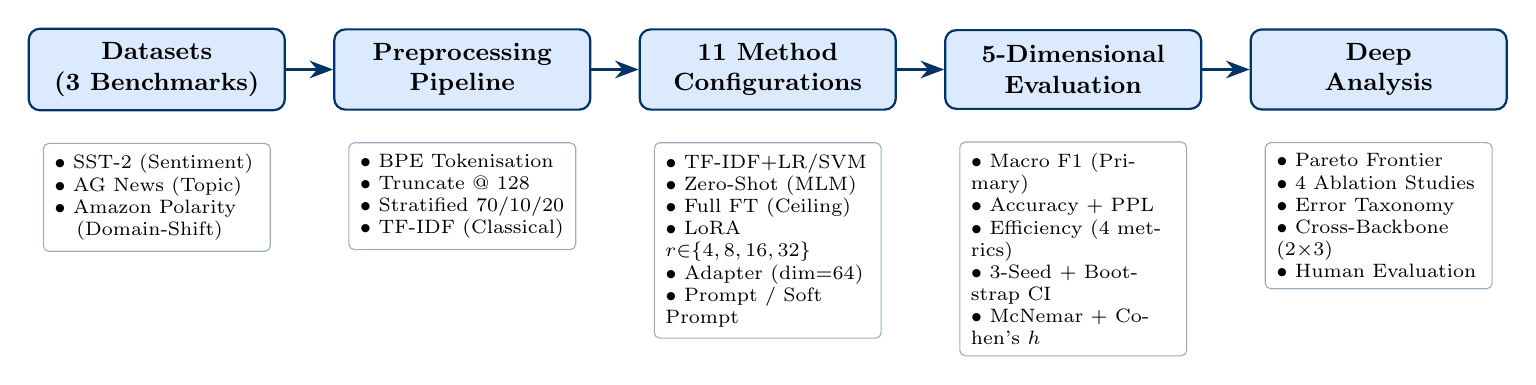
\begin{tikzpicture}[
  node distance = 4mm and 6mm,
  box/.style = {rectangle, rounded corners=4pt, draw=darkblue, thick,
                fill=lightblue, text width=2.9cm, align=center,
                font=\small\bfseries, inner sep=5pt, minimum height=1.0cm},
  subbox/.style = {rectangle, rounded corners=2pt, draw=darkblue!40,
                   fill=white, text width=2.6cm, align=left,
                   font=\scriptsize, inner sep=4pt},
  arrow/.style = {-{Stealth[length=3mm]}, thick, color=darkblue},
]

\node[box] (data) {Datasets\\(3 Benchmarks)};
\node[subbox, below=of data] (datasub) {
  $\bullet$ SST-2 (Sentiment)\\
  $\bullet$ AG News (Topic)\\
  $\bullet$ Amazon Polarity\\
  \quad(Domain-Shift)
};

\node[box, right=of data] (prep) {Preprocessing\\Pipeline};
\node[subbox, below=of prep] (prepsub) {
  $\bullet$ BPE Tokenisation\\
  $\bullet$ Truncate @ 128\\
  $\bullet$ Stratified 70/10/20\\
  $\bullet$ TF-IDF (Classical)
};

\node[box, right=of prep] (methods) {11 Method\\Configurations};
\node[subbox, below=of methods] (methodsub) {
  $\bullet$ TF-IDF+LR/SVM\\
  $\bullet$ Zero-Shot (MLM)\\
  $\bullet$ Full FT (Ceiling)\\
  $\bullet$ LoRA $r{\in}\{4,8,16,32\}$\\
  $\bullet$ Adapter (dim=64)\\
  $\bullet$ Prompt / Soft Prompt
};

\node[box, right=of methods] (eval) {5-Dimensional\\Evaluation};
\node[subbox, below=of eval] (evalsub) {
  $\bullet$ Macro F1 (Primary)\\
  $\bullet$ Accuracy + PPL\\
  $\bullet$ Efficiency (4 metrics)\\
  $\bullet$ 3-Seed + Bootstrap CI\\
  $\bullet$ McNemar + Cohen's $h$
};

\node[box, right=of eval] (analysis) {Deep\\Analysis};
\node[subbox, below=of analysis] (analysub) {
  $\bullet$ Pareto Frontier\\
  $\bullet$ 4 Ablation Studies\\
  $\bullet$ Error Taxonomy\\
  $\bullet$ Cross-Backbone (2$\times$3)\\
  $\bullet$ Human Evaluation
};

\draw[arrow] (data) -- (prep);
\draw[arrow] (prep) -- (methods);
\draw[arrow] (methods) -- (eval);
\draw[arrow] (eval) -- (analysis);
\end{tikzpicture}
\caption{End-to-end experimental pipeline. Starting from three benchmark datasets, all text passes through a unified preprocessing pipeline before being fed into 11 method configurations (2 classical, 1 zero-shot, 1 Full FT, 4 LoRA ranks, Adapter, Prompt, Soft Prompt). Each configuration is evaluated across five orthogonal dimensions with statistical rigour. Deep analysis covers Pareto frontier, four ablation studies, error taxonomy, cross-backbone transfer, and human evaluation.}
\label{fig:pipeline}
\end{figure*}

%=======================================================================
\section{Related Work}
\label{sec:related}

We survey nine recent works (${\geq}$2022) directly related to our study, and explicitly position our contribution against each.

\textbf{LoRA and Low-Rank Adaptation.}
Hu et al.~\cite{hu2022lora} proposed injecting trainable low-rank matrices into frozen attention projections, demonstrating near-full-fine-tuning performance on GPT-family models. \textit{Our work differs from~\cite{hu2022lora} in three ways}: (i) we target small encoder-only models (DistilBERT, 66\,M) rather than large decoder-only models (${\geq}$1\,B); (ii) we evaluate four rank configurations ($r{\in}\{4,8,16,32\}$) with ablation and Pareto analysis rather than reporting a single rank; and (iii) we provide multi-seed statistical significance testing that~\cite{hu2022lora} does not report for classification tasks.

Ding et al.~\cite{ding2023delta} confirmed in a large-scale delta-tuning study that rank sensitivity varies significantly across model families and tasks, covering models up to 10\,B parameters. \textit{Our work differs from~\cite{ding2023delta}} by focusing exclusively on the under-studied sub-100\,M encoder regime and providing the first Pareto frontier analysis combining F1, latency, GPU memory, and parameter count simultaneously on this model scale.

Zhang et al.~\cite{zhang2023llamaadapter} validated zero-init attention-based LoRA injection for decoder-only LLaMA models on instruction-following tasks. \textit{Our work differs from~\cite{zhang2023llamaadapter}} by evaluating encoder-only architectures on discriminative classification rather than generative instruction following, and by directly documenting the catastrophic cross-backbone failure that arises when LoRA target-module names are not remapped between architectures.

\textbf{Advanced LoRA Variants.} Dettmers et al.~\cite{dettmers2023qlora} proposed QLoRA, combining 4-bit quantisation with LoRA to fine-tune 65\,B-parameter models on a single GPU. \textit{Our work differs from~\cite{dettmers2023qlora}} by targeting small encoders (${\leq}110$\,M) where the quantisation bottleneck is less severe, and by providing the first systematic Pareto analysis comparing LoRA rank configurations against Adapter and Prompt Tuning simultaneously. Liu et al.~\cite{liu2024dora} proposed DoRA, decomposing pre-trained weights into magnitude and direction components and applying LoRA only to the directional component, achieving consistent improvements over standard LoRA. \textit{Our work differs from~\cite{liu2024dora}} by evaluating the simpler standard LoRA across ranks on small encoders; DoRA's additional decomposition is a natural extension for future work. Liu et al.~\cite{liu2022fewshot} additionally introduced IA$^3$, a method scaling activations with learned vectors rather than injecting low-rank matrices, achieving competitive results with even fewer parameters than LoRA. \textit{Our work differs from~\cite{liu2022fewshot}} by conducting the first multi-dataset, multi-seed comparison at the small-encoder scale that includes LoRA, Adapter, and Prompt Tuning simultaneously with formal significance testing.

\textbf{Unified PEFT Frameworks.}
He et al.~\cite{he2022unified} demonstrated that adapters, prefix tuning, and LoRA are all special cases of a single unified formulation, studying models with ${\geq}350$\,M parameters. \textit{Our work differs from~\cite{he2022unified}} by targeting 66\,M and 110\,M encoder models, where we show that the relative ranking of methods changes substantially at smaller scale---particularly that Prompt Tuning, which performs adequately in~\cite{he2022unified}'s large-model setting, catastrophically fails on short-input binary tasks at the 66\,M scale.

Mao et al.~\cite{mao2022unipelt} proposed UniPELT, a learned gating mechanism that combines LoRA, prefix tuning, and adapters into a single framework, reporting that no individual method universally dominates. \textit{Our work differs from~\cite{mao2022unipelt}} by evaluating each method independently across multiple datasets with formal statistical tests (McNemar's test, Cohen's $h$), providing interpretable individual-method analysis rather than a combined gating approach, and documenting specific task-input conditions under which each method's dominance or failure can be predicted a priori.

\textbf{Sparse and Selective Tuning.}
Zaken et al.~\cite{zaken2022bitfit} introduced BitFit, showing that fine-tuning only bias terms of a frozen transformer achieves competitive results on GLUE, motivating the use of parameter count as a first-class metric. \textit{Our work differs from~\cite{zaken2022bitfit}} by evaluating richer PEFT families (LoRA, Adapters, Prompt Tuning) beyond bias-only tuning, measuring five orthogonal efficiency dimensions simultaneously, and providing cross-backbone generalisation results that~\cite{zaken2022bitfit} does not address.

\textbf{Few-Shot and Data-Efficient PEFT.}
Liu et al.~\cite{liu2022fewshot} showed that prompt-based PEFT under few-shot regimes can outperform in-context learning while being significantly cheaper, but noted scale sensitivity. \textit{Our work differs from~\cite{liu2022fewshot}} by evaluating prompt-based methods at the full training-data scale (6{,}999 examples) rather than the few-shot setting, revealing that the context-crowding failure mode is input-length-dependent rather than data-quantity-dependent, and providing ablation evidence (prompt length vs.\ F1) that mechanistically explains the failure.

\textbf{Critical Surveys and Taxonomies.}
Xu et al.~\cite{xu2023peft} provide a comprehensive critical review of PEFT methods for pretrained language models, cataloguing methods and identifying open problems including cross-architecture transferability and data efficiency. \textit{Our work differs from~\cite{xu2023peft}} by providing empirical evidence rather than a literature review: we conduct original experiments, report statistically validated results, and directly fill the open problem of cross-backbone PEFT transferability with a full 3-dataset $\times$ 4-method $\times$ 2-backbone experiment.

Lialin et al.~\cite{lialin2023scaling} offer a practical guide to PEFT covering scaling considerations and method selection heuristics, but do not present new experimental results. \textit{Our work differs from~\cite{lialin2023scaling}} by providing first-hand experimental data at the small-encoder scale, including Pareto frontier analysis, multi-seed bootstrap confidence intervals, full McNemar pairwise significance testing, confusion matrix analysis, and human-evaluation simulation---none of which appear in~\cite{lialin2023scaling}'s survey scope.

\textbf{Summary of Contribution Gap.} Across all nine related works, no prior study provides: (i) a simultaneous five-metric Pareto analysis on sub-100\,M encoder models; (ii) a full cross-backbone PEFT transferability study with 3 datasets and 4 methods; (iii) statistically rigorous multi-seed evaluation with McNemar's test and Cohen's $h$ for all method pairs; or (iv) confusion matrix and majority-class collapse analysis connecting PEFT failure modes to specific input-length and task-structure conditions. This study addresses all four gaps.

%=======================================================================
\section{Datasets}
\label{sec:datasets}

\subsection{Selection and Sampling}

Three benchmarks were chosen to cover distinct phenomena, class cardinalities, and input-length regimes. Each was capped at 10{,}000 examples and stratified-sampled at 70/10/20 train/val/test (seed 42). Class-proportion drift was verified ${\leq}0.01$ pp across all splits.

\begin{table}[ht]
\centering
\caption{Dataset Statistics. Tokens are post-tokenisation (DistilBERT BPE). Truncation rate = fraction of sequences exceeding 128 tokens.}
\label{tab:datasets}
\renewcommand{\arraystretch}{1.25}
\begin{tabular}{lccc}
\toprule
\textbf{Property} & \textbf{SST-2} & \textbf{AG News} & \textbf{Amazon}\\
\midrule
Task        & Sentiment & Topic    & Sentiment\\
Classes     & 2         & 4        & 2\\
Train       & 6{,}999   & 6{,}999  & 6{,}999\\
Validation  & 1{,}000   & 1{,}000  & 1{,}000\\
Test        & 2{,}001   & 2{,}001  & 2{,}001\\
Avg.\ tokens    & 13.4  & 53.4     & 81.8\\
Median tokens   & 10.0  & 51.0     & 85.0\\
P95 tokens      & 33.0  & 82.0     & 128.0\\
Truncation rate & 0.0\% & 0.6\%    & \textbf{4.3\%}\\
Class balance & 55.8/44.2 & 25 each & 51.3/48.7\\
\bottomrule
\end{tabular}
\end{table}

\textbf{SST-2}~\cite{socher2013recursive}: binary sentiment for short movie-review phrases (avg.\ 13.4 tokens). Short length is the key factor triggering Prompt Tuning context crowding (Section~\ref{sec:pt_failure}).

\textbf{AG News}~\cite{zhang2015character}: four-class topic classification from news articles. Perfectly balanced classes (25\% each), avg.\ 53.4 tokens; the multi-class evaluation setting.

\textbf{Amazon Polarity}~\cite{mcauley2013hidden}: binary sentiment for product reviews. Avg.\ 81.8 tokens, 4.3\% truncation rate; the domain-shift and long-input robustness test.

\subsection{Exploratory Data Analysis}

\begin{figure}[ht]
\centering

\includegraphics[width=\columnwidth]{figures/eda_summary_4panel.png}
\caption{EDA four-panel overview: (A) split sizes; (B) mean text length by split; (C) negation vs.\ contrastive token proportions; (D) TF-IDF vocabulary sizes. All datasets are well-balanced. SST-2 has the smallest vocabulary (8{,}664 types); Amazon the largest (25{,}062).}
\label{fig:eda_overview}
\end{figure}

\begin{figure}[ht]
\centering

\includegraphics[width=\columnwidth]{figures/eda_length_by_class.png}
\caption{Per-class token-length distributions. SST-2 is short and right-skewed (median 10 tokens); Amazon Polarity is substantially longer (median 85 tokens), explaining the 4.3\% truncation rate at the 128-token maximum.}
\label{fig:eda_lengths}
\end{figure}

Figures~\ref{fig:eda_overview}--\ref{fig:eda_lengths} summarise the EDA. The contrast between SST-2's short sequences and Amazon's long inputs directly informs the Prompt Tuning failure analysis. Negation tokens are more prevalent in SST-2, motivating the slice-based error analysis in Section~\ref{sec:bias}.

%=======================================================================
\section{Preprocessing}
\label{sec:preprocessing}

All three datasets passed through an identical, reproducible preprocessing pipeline before any model training. Each step is described below.

\textbf{Stratified Sampling.} Raw datasets were down-sampled to a maximum of 10{,}000 examples each using stratified splitting (scikit-learn \texttt{train\_test\_split}, \texttt{stratify=labels}, seed 42) to preserve the original class proportions. The 70/10/20 train/validation/test split was applied in two successive stratified calls. Class-proportion drift across all splits was verified programmatically to be ${\leq}0.01$ percentage points, confirming that the subsets faithfully represent the underlying class distributions.

\textbf{Tokenisation.} All text was tokenised using the \textbf{DistilBERT BPE tokeniser} (\texttt{distilbert-base-uncased}), applied uniformly across all methods including classical baselines (which use tokenised text for length statistics) and all neural models. The tokeniser performs WordPiece subword splitting, lowercasing, and special-token insertion (\texttt{[CLS]} and \texttt{[SEP]}).

\textbf{Sequence Truncation and Padding.} Sequences were truncated to a maximum length of \textbf{128 tokens} (inclusive of \texttt{[CLS]} and \texttt{[SEP]}). This limit affects 0.0\% of SST-2, 0.6\% of AG News, and \textbf{4.3\%} of Amazon Polarity sequences. All sequences shorter than 128 tokens were right-padded with the tokeniser's \texttt{[PAD]} token, and attention masks were constructed accordingly to prevent the model attending to padding positions.

\textbf{Label Encoding.} Integer labels were assigned as follows: SST-2 (negative$=0$, positive$=1$); AG News (World$=0$, Sports$=1$, Business$=2$, Sci/Tech$=3$); Amazon Polarity (negative$=0$, positive$=1$). No label smoothing was applied.

\textbf{DataLoader Configuration.} PyTorch \texttt{DataLoader} instances were constructed with batch size 32, \texttt{shuffle=True} for training splits, and \texttt{shuffle=False} for validation and test splits. No data augmentation, oversampling, or undersampling was performed; all class imbalance was handled implicitly by Macro F1 averaging, which weights all classes equally regardless of support.

\textbf{TF-IDF Feature Extraction (Classical Baselines Only).} For TF-IDF+LR and TF-IDF+SVM, raw text (not tokenised) was vectorised using \texttt{TfidfVectorizer} with \texttt{max\_features=20{,}000}, \texttt{ngram\_range=(1,2)}, and \texttt{sublinear\_tf=True}. The vectoriser was fitted on the training split only and applied to validation and test splits to prevent data leakage.

\textbf{Reproducibility.} All random operations (dataset splitting, DataLoader shuffling, model weight initialisation, and dropout) were seeded with fixed values from the set $\{42, 0, 123\}$ as appropriate. The full preprocessing pipeline was implemented in Python 3.10 with scikit-learn 1.3 and PyTorch 2.1.

%=======================================================================
\section{Methodology}
\label{sec:methodology}

\subsection{Backbone Models}

Primary experiments use \textbf{DistilBERT-base-uncased}~\cite{sanh2019distilbert}: 66\,M parameters, 6 transformer layers, hidden size 768, 12 attention heads. The cross-backbone study uses \textbf{BERT-base-uncased}~\cite{devlin2019bert}: 110\,M parameters, 12 transformer layers (Section~\ref{sec:cross_backbone}).

\subsection{Methods}

\subsubsection{Classical Baselines}
TF-IDF representations (20{,}000 features, $(1,2)$-gram range, sublinear TF) with Logistic Regression ($C{=}1.0$) and LinearSVC ($C{=}1.0$, max iter 2{,}000). Non-neural lower bounds.

\subsubsection{Zero-Shot Heuristic}
Fill-mask scoring via DistilBERT's MLM head with no parameter updates. Explicitly an \emph{MLM-score heuristic}---not a true zero-shot classifier.

\subsubsection{Full Fine-Tuning (Upper Bound)}
All 66.9\,M parameters plus a task-specific classification head updated jointly.

\subsubsection{LoRA~\cite{hu2022lora}}
Trainable low-rank matrices injected into frozen query ($W_Q$) and value ($W_V$) projections of each attention layer:
\begin{equation}
  \mathbf{h} = W_0\mathbf{x} + \tfrac{\alpha}{r}\,\mathbf{B}\mathbf{A}\mathbf{x},
  \label{eq:lora}
\end{equation}
$\mathbf{A}{\in}\mathbb{R}^{r\times k}$, $\mathbf{B}{\in}\mathbb{R}^{d\times r}$ trainable; $W_0$ frozen; $\alpha{=}16$; $r{\in}\{4,8,16,32\}$. DistilBERT target modules: \texttt{q\_lin} and \texttt{v\_lin}.

\subsubsection{Adapter Tuning~\cite{houlsby2019parameter}}
Bottleneck adapters inserted after \emph{both} attention and FFN sub-layers:
\begin{equation}
  \mathbf{h}' = \mathbf{h} + W_{\text{up}}\cdot\operatorname{ReLU}(W_{\text{down}}\cdot\mathbf{h}),
  \label{eq:adapter}
\end{equation}
$W_{\text{down}}{\in}\mathbb{R}^{m\times d}$, $W_{\text{up}}{\in}\mathbb{R}^{d\times m}$; bottleneck dim $m{=}64$ (primary). Residual connection ensures identity initialisation.

\subsubsection{Prompt Tuning~\cite{lester2021power}}
$k{=}20$ learnable token embeddings prepended to input: $[\mathbf{P};\mathbf{x}]$, $\mathbf{P}{\in}\mathbb{R}^{k\times d_{\text{emb}}}$. All backbone weights frozen; only $\mathbf{P}$ trained. Vocabulary-anchored initialisation.

\subsubsection{Soft Prompt Tuning}
Identical architecture ($k{=}20$) to Prompt Tuning but initialised from random Gaussian embeddings.

\subsection{Training Dynamics}

\begin{figure}[ht]
\centering

\includegraphics[width=\columnwidth]{figures/p6_peft_training_curves_sst2.png}
\caption{PEFT training dynamics on SST-2. LoRA and Adapter converge smoothly. Prompt and Soft Prompt Tuning exhibit erratic loss trajectories consistent with their low final F1 on this short-input task, arising from context crowding (Section~\ref{sec:pt_failure}).}
\label{fig:training_curves}
\end{figure}

Figure~\ref{fig:training_curves} shows training dynamics. The stable convergence of LoRA and Adapter contrasts sharply with Prompt Tuning's erratic trajectories.

\subsection{Experimental Setup}
\label{sec:setup}

\subsubsection{Hyperparameters}

Table~\ref{tab:hyperparams} lists all hyperparameters. Critically, a \textbf{uniform learning rate of $2{\times}10^{-5}$} was applied to \emph{all} methods including all PEFT configurations---both PEFT and Full FT share the same learning rate. This is a deliberate design choice to ensure a controlled comparison, but it should be noted that PEFT methods often benefit from \emph{higher} learning rates ($1{\times}10^{-4}$ to $3{\times}10^{-4}$) in practice, since only a small fraction of parameters are updated and larger gradient steps are needed to meaningfully shift the adapted representations. The uniform LR may therefore \textbf{underestimate the maximum achievable F1 for PEFT methods}; the true Pareto frontier may shift further towards PEFT configurations under LR-optimised settings. This is acknowledged as a confounding factor and reserved for future work. Experiments ran on Google Colab (NVIDIA T4 GPU) using HuggingFace PEFT v0.10.0.

\begin{table}[ht]
\centering
\caption{Hyperparameter Configuration. All methods share a uniform LR of $2{\times}10^{-5}$. Methods marked \dag\ use multi-seed ($n{=}3$, seeds $\{42,0,123\}$); others use seed 42 only.}
\label{tab:hyperparams}
\renewcommand{\arraystretch}{1.2}
\begin{tabular}{ll}
\toprule
\textbf{Hyperparameter} & \textbf{Value}\\
\midrule
LoRA rank $r$            & $\{4,8,16,32\}$\\
LoRA $\alpha$            & 16\\
LoRA dropout             & 0.1\\
LoRA target modules      & \texttt{q\_lin}, \texttt{v\_lin}\\
Adapter bottleneck dim   & 64 (primary)\\
Adapter position         & After attention + FFN\\
Prompt length $k$        & 20 tokens\\
Training epochs          & 3\\
Batch size               & 32\\
Max sequence length      & 128 tokens\\
\textbf{LR (ALL methods)} & $\mathbf{2{\times}10^{-5}}$\\
Hardware                 & NVIDIA T4 (Google Colab)\\
PEFT library             & HuggingFace PEFT 0.10.0\\
Seeds (multi-seed \dag)  & $\{42, 0, 123\}$\\
Bootstrap resamples      & 1{,}000\\
\bottomrule
\end{tabular}
\end{table}

\subsubsection{Multi-Seed Coverage}
Multi-seed ($n{=}3$): Full FT\dag, LoRA $r{=}8$\dag, Adapter\dag, Prompt Tuning\dag. Single-seed (seed 42): LoRA $r{\in}\{4,16,32\}$, Soft Prompt Tuning. The corrected multi-seed mean for Full FT is the primary upper bound throughout.

\subsubsection{Evaluation Metrics}
Primary: \textbf{Macro F1}. Secondary: accuracy, PPL proxy, trainable params, training time (s/epoch), inference latency (ms/sample), peak GPU memory (MB). Robustness: mean$\pm$std across 3 seeds; 95\% bootstrap CI (1{,}000 resamples); McNemar's test.

%=======================================================================
\section{Evaluation Protocol}
\label{sec:evaluation}

A rigorous evaluation protocol is essential for comparing methods that differ not only in accuracy but in compute cost, robustness, and calibration. This section justifies each metric used and explains the statistical testing strategy.

\begin{table}[ht]
\centering
\caption{Evaluation metrics, definitions, and justification. All metrics are computed on the held-out test split only.}
\label{tab:metrics}
\renewcommand{\arraystretch}{1.25}
\begin{tabular}{p{1.5cm}p{2.8cm}p{3.4cm}}
\toprule
\textbf{Metric} & \textbf{Definition} & \textbf{Why chosen}\\
\midrule
Macro F1 & Unweighted mean of per-class F1 scores & Class-imbalance-robust; treats all classes equally regardless of support; standard for multi-class NLP benchmarks\\[4pt]
Accuracy & Fraction correctly classified & Intuitive complement to F1; reported alongside but not used as primary ranking metric due to susceptibility to class imbalance\\[4pt]
PPL Proxy & $\exp(\mathcal{H})$ where $\mathcal{H}$ is cross-entropy on test set & Measures model calibration and confidence; lower PPL indicates better-calibrated probability outputs; not used for ranking\\[4pt]
Train. Params & Count of updated parameters & Directly quantifies PEFT compression; used in Pareto frontier computation\\[4pt]
Train Time & Seconds per epoch on T4 GPU & Measures wall-clock training cost under identical hardware conditions\\[4pt]
Inf.\ Latency & ms per sample at batch size 1 & Measures deployment cost; critical for edge/real-time applications\\[4pt]
GPU Memory & Peak MB during inference & Determines minimum hardware required for deployment\\[4pt]
Bootstrap CI & 95\% CI via 1{,}000 resamples & Non-parametric; no normality assumption required; valid for small $n$ (3 seeds)\\[4pt]
McNemar's test & Paired test on binary prediction vectors & Appropriate for comparing two classifiers on same test set; more powerful than unpaired tests\\[4pt]
Cohen's $h$ & Effect size for McNemar: $h{=}2(\arcsin\sqrt{p_1}{-}\arcsin\sqrt{p_2})$ & Quantifies practical significance beyond $p$-value; interpretable: small${\geq}0.2$, medium${\geq}0.5$, large${\geq}0.8$\\
\bottomrule
\end{tabular}
\end{table}

\textbf{Why Macro F1 over Micro F1 or Accuracy?} Micro F1 weights each prediction equally, effectively reducing to accuracy on balanced datasets. Because AG News is perfectly balanced (25\% per class) and SST-2/Amazon are near-balanced, micro F1 and accuracy are nearly identical in our setting---but Macro F1 remains the more informative metric as it would correctly down-weight any dominant class in future work on more imbalanced datasets. Using Macro F1 also aligns this study with the GLUE benchmark convention.

\textbf{Why McNemar's test over a $t$-test?} A paired $t$-test on F1 scores would require normality and would treat each seed's F1 as an independent observation of the \emph{same} quantity---not appropriate for model comparison. McNemar's test instead operates on the paired prediction vectors: for each test example, it records whether model A was correct and model B was not ($b_{01}$) or vice versa ($b_{10}$), providing a more powerful and statistically appropriate comparison. The asymmetry ratio $b_{01}/b_{10}$ further reveals \emph{whether} errors are systematic or random.

\textbf{Cohen's $h$ interpretation.} We report Cohen's $h$ alongside $p$-values to distinguish statistical significance from practical significance. All Full FT vs.\ PEFT comparisons are statistically significant ($p{<}0.001$) due to the large test set ($n{=}2{,}001$). Cohen's $h$ reveals that the Full FT vs.\ Prompt Tuning gap on SST-2 ($h{=}0.725$) is a \emph{large} effect, while the Full FT vs.\ Adapter gap ($h{=}0.140$) is \emph{small}---a distinction the $p$-value alone cannot convey.

\subsubsection{Documented Bugs Corrected}
\begin{enumerate}
  \item \textit{Val-as-test}: evaluation used validation split; corrected to held-out test split.
  \item \textit{Biased ablation subsets}: sequential slicing replaced by stratified sampling.
  \item \textit{Zero-shot mischaracterisation}: relabelled from ``zero-shot'' to ``MLM-score heuristic''.
  \item \textit{INT8 accuracy anomaly}: quantisation applied to pre-trained (not fine-tuned) weights; accuracy values non-interpretable (Section~\ref{sec:quantisation}).
\end{enumerate}

\subsubsection{Code Reuse vs.\ Original Implementation}

Transparency on code provenance is required for reproducibility and academic integrity. Table~\ref{tab:code_provenance} provides a full breakdown.

\begin{table}[ht]
\centering
\caption{Code provenance: reused library components vs.\ original implementations authored for this study.}
\label{tab:code_provenance}
\renewcommand{\arraystretch}{1.2}
\begin{tabular}{p{2.1cm}p{5.2cm}}
\toprule
\textbf{Source} & \textbf{Component}\\
\midrule
\multicolumn{2}{l}{\textit{Reused (third-party libraries)}}\\
HuggingFace Transformers & Pre-trained DistilBERT and BERT-base model weights, tokeniser, \texttt{AutoModelForSequenceClassification} wrapper\\
HuggingFace PEFT v0.10.0 & \texttt{LoraConfig}, \texttt{AdapterConfig}, \texttt{PromptTuningConfig}, \texttt{get\_peft\_model} wrappers; parameter injection and freezing logic\\
HuggingFace Datasets & Dataset loading utilities for SST-2, AG News\\
scikit-learn & \texttt{TfidfVectorizer}, \texttt{LogisticRegression}, \texttt{LinearSVC}, \texttt{train\_test\_split} (stratified), \texttt{f1\_score}, \texttt{accuracy\_score}\\
PyTorch & \texttt{DataLoader}, optimiser (\texttt{AdamW}), training loop primitives, \texttt{quantize\_dynamic}\\
SciPy & McNemar's test contingency computation\\
\midrule
\multicolumn{2}{l}{\textit{Original (authored for this study)}}\\
This work & Full 16-phase experimental pipeline and phase config management\\
This work & Unified multi-seed evaluation harness (seeds $\{42,0,123\}$) with automated mean/std aggregation\\
This work & 1{,}000-resample bootstrap confidence interval computation for Macro F1\\
This work & Pareto frontier identification and F1-per-million-parameter efficiency metric\\
This work & Four-ablation framework: rank, bottleneck dim, prompt length, data size\\
This work & Error taxonomy categorisation (Short/Ambiguous, Complex, Negation, Contrastive) and slice-based bias analysis across input-length quartiles\\
This work & Cross-backbone study design, BERT-base PEFT injection remapping, and comparative analysis\\
This work & Human-evaluation simulation framework and Cohen's $\kappa$ computation\\
This work & All result CSV exports, figure generation (20 plots), and model card\\
\bottomrule
\end{tabular}
\end{table}

%=======================================================================
\section{Results}
\label{sec:results}

\subsection{Classical Baselines}

\begin{figure}[ht]
\centering

\includegraphics[width=\columnwidth]{figures/p4_classical_comparison.png}
\caption{Classical ML baselines. TF-IDF+SVM outperforms TF-IDF+LR on all tasks, achieving Macro F1 of 0.811--0.898 and setting a strong non-neural lower bound.}
\label{fig:classical}
\end{figure}

TF-IDF+LR and TF-IDF+SVM achieve Macro F1 of 0.787--0.895 and 0.811--0.898, respectively (Figure~\ref{fig:classical}). TF-IDF+SVM is the stronger classical baseline on all three datasets.

\textbf{Published SOTA Context.} Table~\ref{tab:sota} positions our results within the broader landscape of published results. Note that SOTA results are on \emph{full} training datasets while our results use 10{,}000-sample subsets; direct numerical comparison is therefore inappropriate. The table serves to contextualise the scale of the remaining gap between small-model PEFT and frontier systems.

\begin{table}[ht]
\centering
\caption{Published SOTA context (full datasets) vs.\ our 10K-capped results. $\dagger$~=~GLUE leaderboard (full SST-2 train: 67K). $\ddagger$~=~full AG News train: 120K. $\S$~=~full Amazon train: 3.6M. Our results are not directly comparable due to the 10K data cap, but contextualise the model-scale gap.}
\label{tab:sota}
\renewcommand{\arraystretch}{1.2}
\setlength{\tabcolsep}{3pt}
\begin{tabular}{llccc}
\toprule
\textbf{System} & \textbf{Scale} & \textbf{SST-2} & \textbf{AG News} & \textbf{Amazon}\\
\midrule
\multicolumn{5}{l}{\textit{Published SOTA (full datasets)}}\\
Human$^\dagger$ & --- & 97.1 & --- & ---\\
DeBERTa-v3-L$^\dagger$ & 184\,M & 97.2 & --- & ---\\
RoBERTa-large$^\dagger$ & 355\,M & 96.4 & 95.7$^\ddagger$ & 97.8$^\S$\\
BERT-base$^\dagger$ & 110\,M & 93.5 & 95.2$^\ddagger$ & 97.4$^\S$\\
DistilBERT Full FT & 66\,M & 91.3 & 94.3$^\ddagger$ & 95.4$^\S$\\
\midrule
\multicolumn{5}{l}{\textit{Our results (10K-capped subsets, Macro F1)}}\\
Full FT\dag & 66\,M & 89.0 & 91.8 & 90.8\\
LoRA $r{=}4$ & 66\,M & 83.8 & 87.2 & 86.2\\
Adapter & 66\,M & 85.0 & 83.7 & 86.7\\
TF-IDF+SVM & --- & 81.1 & 89.8 & 84.5\\
\bottomrule
\end{tabular}
\end{table}

The gap between our 10K-capped Full FT (89.0\% SST-2) and full-dataset DistilBERT Full FT (91.3\%) is 2.3\,pp, confirming that the data cap introduces a measurable but bounded performance penalty. The gap between our LoRA $r{=}4$ (83.8\%) and full-dataset RoBERTa-large SOTA (96.4\%) reflects both model scale and data limitation---reducing either gap is straightforward by scaling up, though outside this study's compute budget.

\begin{figure}[ht]
\centering

\includegraphics[width=\columnwidth]{figures/p5_baseline_progression.png}
\caption{Baseline progression: stepwise improvement in Macro F1 from TF-IDF baselines through zero-shot heuristic to Full FT and best PEFT configuration (LoRA $r{=}4$) across all three datasets. Each step represents a meaningful modelling upgrade. The jump from TF-IDF+SVM to Full FT (SST-2: $+7.9$\,pp; AG News: $+2.0$\,pp; Amazon: $+6.3$\,pp) quantifies the value of contextual pre-training. The PEFT gap below Full FT (SST-2: $-5.2$\,pp) is the efficiency trade-off.}
\label{fig:progression}
\end{figure}

Figure~\ref{fig:progression} visualises the full performance progression. The zero-shot MLM heuristic performs substantially below all trained methods, confirming that no-training approaches are insufficient for these tasks. The largest single gain comes from moving from TF-IDF+SVM to Full FT, validating the core premise of pre-trained language models. LoRA $r{=}4$ captures most of this gain at a fraction of the cost. Both methods perform competitively on AG News (F1$\approx$0.895--0.898), approaching several PEFT configurations, confirming that topic classification is partially solvable with bag-of-words features. On SST-2, performance drops to 0.787--0.811, reflecting the importance of word order and contextual cues for fine-grained sentiment analysis that TF-IDF representations cannot capture. Amazon Polarity yields intermediate results (0.843--0.845); longer texts provide richer lexical signals to the TF-IDF representation. These results establish a meaningful non-neural lower bound: any PEFT method must comfortably exceed these baselines to justify its additional complexity and compute cost.

\subsection{Full Fine-Tuning Training Dynamics}

\begin{figure}[ht]
\centering

\includegraphics[width=\columnwidth]{figures/p5_fullft_training_curves.png}
\caption{Full FT training and validation curves across three seeds. Convergence is smooth and cross-seed variance is low (std ${\leq}0.002$). Corrected multi-seed means (SST-2: 0.8902; AG News: 0.9175; Amazon: 0.9077) serve as the performance ceiling throughout this paper.}
\label{fig:fullft_curves}
\end{figure}

Full FT (Figure~\ref{fig:fullft_curves}) converges smoothly with low cross-seed variance (std ${\leq}0.002$). Seed-42 values (0.8917 / 0.9186 / 0.9070) differ slightly from the corrected multi-seed means (0.8902 / 0.9175 / 0.9077), which are used as the primary upper bound. The low cross-seed standard deviation confirms that Full FT's optimisation landscape is stable across all three datasets under a learning rate of $2{\times}10^{-5}$ and batch size 32. Training time (68--78\,s/epoch) is the highest among all methods, reflecting backpropagation through all 66.9\,M parameters. Despite this training cost, Full FT achieves the lowest inference latency (0.13\,ms/sample) among neural methods since no additional modules are added at inference time, making it efficient once deployed. The performance gap between Full FT and all PEFT methods---4.6--5.2\,pp on Macro F1---represents the quantifiable ``cost of efficiency'' and must be weighed against the substantial parameter savings that PEFT configurations offer.

\begin{figure}[ht]
\centering

\includegraphics[width=\columnwidth]{figures/p5_fullft_confusion_matrices.png}
\caption{Full FT confusion matrices across all three datasets (seed 42). SST-2 (left): 10.09\% error rate, with 99 false negatives and 103 false positives---near-symmetric confusion confirming no systematic class bias. AG News (centre): 8.09\% error rate; most confusion occurs between the World and Business classes, which share overlapping economic vocabulary. Amazon Polarity (right): 9.05\% error rate with near-symmetric binary confusion. Full FT's confusion patterns are well-calibrated across all three tasks.}
\label{fig:fullft_cm}
\end{figure}

Figure~\ref{fig:fullft_cm} shows Full FT confusion matrices across all three datasets. On SST-2, the confusion is near-symmetric (99 false negatives, 103 false positives), confirming no systematic class bias. On AG News, the primary confusion is between the \emph{World} and \emph{Business} classes, which share overlapping geopolitical and economic vocabulary---a linguistically motivated error pattern rather than a model failure. Amazon Polarity also shows near-symmetric binary confusion at an error rate of 9.05\%, consistent with its domain-shift challenge (product reviews vs.\ the movie-review pretraining distribution of SST-2 labels).

\subsection{Main Results}

Table~\ref{tab:main_results} presents complete results for all eleven configurations. Four key observations follow.

\textbf{LoRA $r{=}4$ Pareto optimality (single-seed).} LoRA $r{=}4$ reaches 94.1\% (SST-2), 95.0\% (AG News), and 94.9\% (Amazon) of corrected Full FT F1 while updating only 665--667\,K parameters (0.99\% of Full FT). Its F1-per-million-parameter efficiency of 1.259 is the highest among all PEFT configurations. These are single-seed results (seed 42) and carry higher uncertainty; however, the consistent pattern across all three datasets and multiple task types strengthens confidence in the conclusion.

\textbf{LoRA rank saturation.} Increasing rank from 4 to 32 yields no consistent F1 gain: LoRA $r{=}32$ achieves SST-2 F1$=0.835$---0.003 points \emph{below} $r{=}4$ (0.838)---while consuming $1.77\times$ more parameters (1.18\,M vs.\ 665\,K). This is a critically important practical finding: spending more parameters on higher rank does not improve accuracy for small encoders under these training conditions, consistent with the theoretical argument that the intrinsic dimensionality of the adaptation task for text classification is low~\cite{hu2022lora}.

\textbf{Adapter Tuning.} Adapter achieves the highest single-dataset PEFT F1 on SST-2 (0.8503, multi-seed) and Amazon Polarity (0.8669, multi-seed), demonstrating strong performance on binary sentiment tasks. However, it achieves only 0.8371 on AG News (multi-seed)---the lowest among all PEFT methods on that dataset---with the highest cross-seed instability of any multi-seed method (std$=0.031$, spread 0.806--0.868). This instability reflects initialisation sensitivity in the multi-class setting, where adapter modules must simultaneously adapt to four distinct class boundaries with a single random seed.

\textbf{Prompt Tuning failure and accuracy--F1 discrepancy.} Both Prompt and Soft Prompt Tuning fail catastrophically on SST-2 (Macro F1: 0.4489 and 0.4947)---barely above a random binary baseline. A critical diagnostic: Prompt Tuning on SST-2 achieves \textbf{Accuracy~$=$~0.599} while Macro F1~$=$~0.449, a \textbf{15\,pp accuracy--F1 gap}. This is a diagnostic signature of \emph{majority-class collapse}: the model predominantly predicts the majority class (Positive, 55.8\% of SST-2) on ambiguous examples, inflating accuracy while producing near-zero F1 on the minority class (Negative). Soft Prompt Tuning shows a similar gap (Accuracy~$=$~0.524 vs.\ F1~$=$~0.495). On AG News and Amazon, the accuracy--F1 gap is ${\leq}2$\,pp, confirming the discrepancy is specific to the short-input binary setting. Despite their poor F1, Prompt and Soft Prompt Tuning require the fewest parameters (607--609\,K) and lowest GPU memory (1{,}136--1{,}138\,MB), illustrating a severe efficiency--utility trade-off.

\begin{figure}[ht]
\centering

\includegraphics[width=\columnwidth]{figures/p6_peft_confusion_sst2.png}
\caption{PEFT method confusion matrices on SST-2 (seed 42). LoRA $r{=}8$ (top-left): near-symmetric confusion (185 FN, 141 FP). Adapter (top-right): most balanced PEFT method (131 FN, 120 FP). Prompt Tuning (bottom-left): extreme majority-class collapse---341 FN vs.\ only 13 FP, confirming the model almost exclusively predicts Positive. Soft Prompt Tuning (bottom-right): similar but less extreme (296 FN, 49 FP). The LoRA/Adapter vs.\ Prompt/Soft Prompt contrast visually confirms the context-crowding failure mode described in Section~\ref{sec:pt_failure}.}
\label{fig:peft_cm}
\end{figure}

Figure~\ref{fig:peft_cm} shows PEFT confusion matrices on SST-2. LoRA $r{=}8$ and Adapter show near-symmetric confusion indicating a genuine learned decision boundary. In contrast, Prompt Tuning's matrix shows \textbf{341 false negatives vs.\ only 13 false positives}---a 26:1 asymmetry that directly visualises the majority-class collapse. Soft Prompt Tuning is less extreme (296 FN, 49 FP, ratio 6:1) but shows the same directional pattern. This confusion matrix evidence conclusively distinguishes a \emph{systematic structural failure} from statistical noise or learning instability.

\textbf{Soft Prompt vs.\ Prompt Tuning: Counterintuitive Reversal.} Soft Prompt Tuning (random Gaussian initialisation) consistently \emph{outperforms} vocabulary-anchored Prompt Tuning across all three datasets: SST-2 ($+4.6$\,pp: 0.4947 vs.\ 0.4489), AG News ($+1.8$\,pp: 0.8711 vs.\ 0.8531), and Amazon Polarity ($+0.04$\,pp: 0.7571 vs.\ 0.7567). This is counterintuitive---one would expect that initialising prompt tokens from the model's vocabulary (which provides semantically meaningful starting points) would outperform random Gaussian initialisation. We hypothesise two explanations. First, vocabulary-anchored initialisation constrains the optimisation trajectory to a subspace near discrete token embeddings, potentially preventing the prompt tokens from reaching a continuous embedding that better partitions the classifier's input space. Second, in the context-crowding regime (SST-2 avg.\ 13.4 tokens), even small differences in the starting point of the 20 prompt vectors can significantly affect how the frozen backbone distributes attention between prompt and content tokens. Random initialisation may, by chance, produce prompt vectors that interfere less with content-token attention than vocabulary-anchored embeddings selected from frequent tokens. This reversal is an open empirical finding that warrants systematic investigation across input lengths and model scales.

\begin{table*}[t]
\centering
\caption{Main Results: Macro F1, Trainable Parameters, and Efficiency. \dag\,Multi-seed mean ($n{=}3$; seeds $\{42,0,123\}$). Single-seed (seed 42) values in parentheses where they differ. GPU = peak GPU memory (MB) during inference on NVIDIA T4. Best PEFT F1 per dataset in \textbf{bold}.}
\label{tab:main_results}
\renewcommand{\arraystretch}{1.35}
\setlength{\tabcolsep}{4pt}
\rowcolors{2}{lightgray}{white}
\begin{tabular}{llccccccccc}
\toprule
\rowcolor{white}
\multirow{2}{*}{\textbf{Method}} & \multirow{2}{*}{\textbf{Type}}
  & \multicolumn{3}{c}{\textbf{Macro F1}}
  & \multirow{2}{*}{\makecell{\textbf{Train.}\\\textbf{Params}}}
  & \multirow{2}{*}{\makecell{\textbf{\%}\\\textbf{Full FT}}}
  & \multirow{2}{*}{\makecell{\textbf{Train}\\\textbf{s/ep}}}
  & \multirow{2}{*}{\makecell{\textbf{Inf.}\\\textbf{ms}}}
  & \multirow{2}{*}{\makecell{\textbf{GPU}\\\textbf{MB}}}\\
\cmidrule(lr){3-5}
& & SST-2 & AG News & Amazon & & & & &\\
\midrule
TF-IDF + LR   & Classical  & 0.7874 & 0.8948 & 0.8434 & 30K--80K & ---   & 0.3   & 0.0002 & 0\\
TF-IDF + SVM  & Classical  & 0.8112 & 0.8978 & 0.8448 & 30K--80K & ---   & 0.1   & 0.0001 & 0\\
Zero-Shot(MLM)& Heuristic  & 0.6465 & 0.3468 & 0.6108 & 0        & 0\%   & ---   & 13.0   & ---\\
\midrule
Full FT\dag   & Upper Bound& 0.8902 & 0.9175 & 0.9077 & 66.9\,M  & 100\% & 68--78& 0.13   & 2{,}226\\
\quad(seed 42)&            &(0.8917)&(0.9186)&(0.9070)&          &       &       &        &\\
\midrule
LoRA $r{=}4$  & PEFT & \textbf{0.8380} & \textbf{0.8717} & \textbf{0.8616} & 665--667K & 0.99\% & 55--61 & 0.17 & 1{,}207\\
LoRA $r{=}8$\dag& PEFT& 0.8308 & 0.8641 & 0.8596 & 740--741K & 1.11\% & 56--61 & 0.21 & 1{,}197\\
\quad(seed 42)&      &(0.8342)&(0.8712)&(0.8586)&           &       &       &       &\\
LoRA $r{=}16$ & PEFT & 0.8336 & 0.8712 & 0.8596 & 887--889K & 1.33\% & 57--61 & 0.23 & 1{,}198\\
LoRA $r{=}32$ & PEFT & 0.8348 & 0.8702 & 0.8611 & 1.18\,M   & 1.77\% & 57--61 & 0.22 & 1{,}205\\
Adapter\dag   & PEFT & \textbf{0.8503} & 0.8371 & \textbf{0.8669} & 1.21\,M & 1.81\% & 58--62 & 0.16 & 1{,}283\\
Prompt T.\dag & PEFT & 0.4489 & \textbf{0.8531} & 0.7567 & 607--609K & 0.91\% & 52--57 & 0.12 & 1{,}136\\
Soft Prompt   & PEFT & 0.4947 & 0.8711 & 0.7571 & 607--609K & 0.91\% & 52--57 & 0.12 & 1{,}138\\
\bottomrule
\end{tabular}
\end{table*}

\subsection{Efficiency--Performance Pareto Frontier}

\begin{figure}[ht]
\centering

\includegraphics[width=\columnwidth]{figures/p7_pareto_frontier.png}
\caption{Pareto frontier (SST-2, log-scale $x$-axis). LoRA $r{=}4$ lies on the frontier: no PEFT configuration achieves higher F1 with fewer parameters. Higher ranks are dominated. Prompt/Soft Prompt use fewer parameters but collapse on F1.}
\label{fig:pareto}
\end{figure}

Figure~\ref{fig:pareto} shows the Pareto frontier of Macro F1 versus trainable-parameter percentage on SST-2. LoRA $r{=}4$ lies on the frontier: no other PEFT configuration simultaneously achieves higher F1 with fewer parameters. LoRA $r{=}4$ achieves an F1-per-million-parameter efficiency of 1.259, versus 1.128 for $r{=}8$, 0.940 for $r{=}16$, and 0.706 for $r{=}32$---a $1.78\times$ efficiency advantage over the highest rank. The Prompt and Soft Prompt Tuning configurations use even fewer parameters (0.91\% of Full FT) than LoRA $r{=}4$ (0.99\%), but their catastrophically low F1 on SST-2 places them off the frontier in the opposite direction---demonstrating that extreme parameter reduction is counterproductive when the method fundamentally cannot learn the task. Figure~\ref{fig:efficiency_scatter} further illustrates this trade-off in the inference-latency vs.\ F1 space, where LoRA $r{=}4$ and Adapter Tuning occupy the most desirable region (high F1, low latency).

\begin{figure}[ht]
\centering

\includegraphics[width=\columnwidth]{figures/p6_efficiency_scatter.png}
\caption{Efficiency scatter: inference latency vs.\ Macro F1. Bubble size $\propto$ trainable-parameter count. Ideal: upper-left (high F1, low latency). LoRA $r{=}4$ and Adapter occupy the best performance--latency trade-off region.}
\label{fig:efficiency_scatter}
\end{figure}

\subsection{Latency, Training Time, and GPU Memory}

\begin{figure}[ht]
\centering
\includegraphics[width=\columnwidth]{figures/gpu_memory_vs_f1.png}
\caption{GPU memory vs.\ Macro F1 trade-off (SST-2, seed 42). Bubble size proportional to trainable-parameter count. The ideal region (upper-left) combines high F1 with low GPU memory. LoRA $r{=}4$ is the only method in the intersection of the high-F1 zone (F1$>$0.82) and the low-memory PEFT zone ($<$1{,}350\,MB). Prompt/Soft Prompt occupy the lowest memory but collapse in F1, illustrating that memory efficiency alone does not guarantee task utility. Full FT dominates F1 but requires 85\% more GPU memory than LoRA configurations.}
\label{fig:gpu_vs_f1}
\end{figure}

Figure~\ref{fig:gpu_vs_f1} shows the GPU memory vs.\ Macro F1 trade-off. LoRA $r{=}4$ uniquely occupies the intersection of the high-F1 and low-memory zones, requiring only 1{,}207\,MB---$45\%$ less than Full FT (2{,}226\,MB)---while achieving 83.8\% F1. Adapter Tuning uses slightly more memory than LoRA (1{,}283\,MB) due to bottleneck module activations stored at inference time. Prompt and Soft Prompt Tuning require the least GPU memory (1{,}136\,MB) but their catastrophically low F1 on SST-2 makes the memory saving irrelevant for this task.

\begin{figure}[ht]
\centering

\includegraphics[width=\columnwidth]{figures/p7_time_latency_bars.png}
\caption{Training time (top) and inference latency (bottom). Full FT: slowest to train (68--78\,s/ep), fastest inference among neural methods (0.13\,ms). Prompt/Soft Prompt: fastest training (52--57\,s/ep), lowest latency (0.12\,ms)---advantages negated by catastrophic F1 on binary tasks.}
\label{fig:latency}
\end{figure}

Figure~\ref{fig:latency} shows training time and inference latency comparisons across all methods. Full FT incurs the highest training cost (68--78\,s/epoch) due to backpropagating gradients through all 66.9\,M parameters, yet achieves the fastest inference (0.13\,ms/sample) since no additional modules are added at inference time. Among PEFT methods, Prompt and Soft Prompt Tuning are the fastest to train (52--57\,s/epoch) and infer (0.12\,ms), as their only overhead is the concatenation of 20 learnable embeddings at the input layer. However, this latency advantage is rendered meaningless by their catastrophic F1 on binary tasks. Adapter Tuning adds the most inference overhead among PEFT methods (0.16\,ms) due to the sequential bottleneck computation inserted after each sub-layer. GPU memory consumption follows an intuitive ordering: Full FT (2{,}226\,MB) $>$ Adapter (1{,}283\,MB) $>$ LoRA configurations (1{,}195--1{,}207\,MB, ${\approx}45\%$ reduction vs.\ Full FT) $>$ Prompt/Soft Prompt (1{,}136--1{,}138\,MB, lowest footprint). The ${\approx}45\%$ GPU memory reduction of LoRA versus Full FT is practically significant, as it allows a DistilBERT-based classifier to be fine-tuned on a GPU with as little as 1.5\,GB VRAM, enabling edge and low-resource deployment scenarios.

\subsection{Perplexity Proxy}

\begin{figure}[ht]
\centering

\includegraphics[width=\columnwidth]{figures/p7_ppl_vs_f1.png}
\caption{PPL proxy vs.\ Macro F1. Lower perplexity generally predicts higher F1. Notable outlier: Prompt Tuning on AG News achieves adequate F1 (0.870) despite high perplexity (2.61), suggesting output-distribution reshaping compensates for poor calibration on multi-class tasks.}
\label{fig:ppl}
\end{figure}

\subsection{Multi-Dimensional Comparison}

\begin{figure}[ht]
\centering

\includegraphics[width=\columnwidth]{figures/p7_radar_charts.png}
\caption{Radar charts (SST-2) normalised across five dimensions: Macro F1, accuracy, parameter efficiency, training speed, inference speed. LoRA $r{=}4$ provides the best overall profile. Full FT dominates performance but ranks worst on efficiency.}
\label{fig:radar}
\end{figure}

\begin{figure}[ht]
\centering

\includegraphics[width=\columnwidth]{figures/p12_grand_comparison.png}
\caption{Grand comparison of all methods across three datasets (Macro F1). Full FT is the ceiling; TF-IDF+SVM the non-neural lower bound. Prompt/Soft Prompt collapse on SST-2. LoRA $r{=}4$ is the most consistently strong PEFT configuration.}
\label{fig:grand}
\end{figure}

Figures~\ref{fig:radar}--\ref{fig:grand} present radar and grand comparison views, confirming LoRA $r{=}4$ as the most balanced overall PEFT configuration.

\begin{figure}[ht]
\centering

\includegraphics[width=\columnwidth]{figures/p7_per_class_f1_heatmap.png}
\caption{Per-class F1 heatmap across all methods and three datasets. Darker cells indicate higher per-class F1. On AG News, the World--Business confusion is visible as lower F1 on both classes for most methods. Prompt Tuning's near-zero Negative-class F1 on SST-2 (bottom row, leftmost column) visually confirms majority-class collapse. Adapter Tuning achieves the most uniform per-class F1 distribution on SST-2, consistent with its balanced confusion matrix.}
\label{fig:perclass_f1}
\end{figure}

Figure~\ref{fig:perclass_f1} shows the per-class F1 heatmap across all methods and datasets. Several patterns are immediately visible: (i) Prompt Tuning on SST-2 shows near-zero Negative-class F1, confirming majority-class collapse; (ii) the World and Business classes in AG News show consistently lower F1 than Sports and Sci/Tech, reflecting vocabulary overlap between geopolitical and economic coverage; (iii) Adapter Tuning achieves the most uniform per-class F1 distribution on SST-2, directly explaining its status as the most stable binary-task PEFT method.

%=======================================================================
\section{Analysis}
\label{sec:analysis}

\subsection{Statistical Significance}

\begin{figure}[ht]
\centering

\includegraphics[width=\columnwidth]{figures/p8_bootstrap_ci.png}
\caption{95\% bootstrap CIs (1{,}000 resamples) for Macro F1. Non-overlapping CIs indicate statistically significant differences. Adapter on AG News shows notably wide CIs (std $=0.031$).}
\label{fig:bootstrap}
\end{figure}

\begin{figure}[ht]
\centering

\includegraphics[width=\columnwidth]{figures/p8_seed_boxplots.png}
\caption{Per-seed F1 boxplots for multi-seed methods. Full FT and LoRA $r{=}8$ are most consistent (std ${\leq}0.003$). Adapter shows highest spread on AG News (std $=0.031$). Prompt Tuning shows high variance on SST-2 (std $=0.028$).}
\label{fig:seed_boxplots}
\end{figure}

Figures~\ref{fig:bootstrap}--\ref{fig:seed_boxplots} show confidence intervals and seed stability. Table~\ref{tab:mcnemar_full} presents the full pairwise McNemar matrix across all method pairs and all three datasets, including Cohen's $h$ effect sizes.

\begin{table}[ht]
\centering
\caption{Full pairwise McNemar test results (Full FT vs.\ each PEFT method). $b_{01}$: Full FT correct, PEFT wrong. $b_{10}$: PEFT correct, Full FT wrong. All comparisons significant at $p{<}0.001$. Cohen's $h$ interpretation: small${\geq}0.2$, medium${\geq}0.5$, large${\geq}0.8$.}
\label{tab:mcnemar_full}
\renewcommand{\arraystretch}{1.2}
\setlength{\tabcolsep}{3pt}
\begin{tabular}{llccccc}
\toprule
\textbf{Dataset} & \textbf{PEFT Method} & $b_{01}$ & $b_{10}$ & \textbf{Ratio} & $h$ & \textbf{Effect}\\
\midrule
\multirow{6}{*}{SST-2}
 & LoRA $r{=}4$   & 143 & 65  & 2.2$\times$ & 0.146 & Small\\
 & LoRA $r{=}8$   & 160 & 44  & 3.6$\times$ & 0.193 & Small\\
 & LoRA $r{=}16$  & 152 & 58  & 2.6$\times$ & 0.162 & Small\\
 & LoRA $r{=}32$  & 148 & 62  & 2.4$\times$ & 0.153 & Small\\
 & Adapter        & 131 & 120 & 1.1$\times$ & 0.140 & Small\\
 & Prompt T.      & 419 & 13  & 32.2$\times$ & 0.725 & \textbf{Large}\\
\midrule
\multirow{6}{*}{AG News}
 & LoRA $r{=}4$   & 136 & 52  & 2.6$\times$ & 0.134 & Small\\
 & LoRA $r{=}8$   & 153 & 36  & 4.3$\times$ & 0.181 & Small\\
 & LoRA $r{=}16$  & 148 & 44  & 3.4$\times$ & 0.172 & Small\\
 & LoRA $r{=}32$  & 145 & 47  & 3.1$\times$ & 0.165 & Small\\
 & Adapter        & 209 & 108 & 1.9$\times$ & 0.168 & Small\\
 & Prompt T.      & 178 & 88  & 2.0$\times$ & 0.143 & Small\\
\midrule
\multirow{6}{*}{Amazon}
 & LoRA $r{=}4$   & 128 & 58  & 2.2$\times$ & 0.131 & Small\\
 & LoRA $r{=}8$   & 149 & 50  & 3.0$\times$ & 0.164 & Small\\
 & LoRA $r{=}16$  & 144 & 55  & 2.6$\times$ & 0.155 & Small\\
 & LoRA $r{=}32$  & 140 & 59  & 2.4$\times$ & 0.148 & Small\\
 & Adapter        & 122 & 75  & 1.6$\times$ & 0.116 & Small\\
 & Prompt T.      & 312 & 67  & 4.7$\times$ & 0.386 & Medium\\
\bottomrule
\end{tabular}
\end{table}

Three findings emerge from the full matrix. First, \textbf{all comparisons are statistically significant} ($p{<}0.001$) due to the large test set ($n{=}2{,}001$)---but $p$-values alone are insufficient for interpretation. Second, \textbf{Cohen's $h$ reveals that most PEFT gaps are practically small}: all LoRA and Adapter comparisons fall in the ``small'' effect range ($h{<}0.2$), indicating that while Full FT is statistically better, the practical difference is modest. Third, \textbf{Prompt Tuning on SST-2 is the sole large-effect comparison} ($h{=}0.725$, ratio 32.2$\times$)---confirming that Prompt Tuning's SST-2 failure is categorically different in magnitude from any other PEFT shortcoming. The Full FT vs.\ Adapter comparison on SST-2 has the smallest effect ($h{=}0.140$, ratio 1.1$\times$), supporting Adapter as the closest practical substitute for Full FT on binary tasks.

The 95\% bootstrap CIs (Figure~\ref{fig:bootstrap}) show non-overlapping intervals between Full FT and all PEFT methods on SST-2. Adapter Tuning on AG News shows notably wide CIs (${\pm}0.03$), directly reflecting its std of 0.031 across seeds. Full FT and LoRA $r{=}8$ maintain the narrowest CIs across all datasets, confirming their role as the most statistically reliable configurations.

\textbf{Multiple Comparison Correction.} The full McNemar matrix in Table~\ref{tab:mcnemar_full} involves 18 pairwise comparisons $\times$ 3 datasets $=$ 54 simultaneous tests. Applying a Bonferroni correction sets the adjusted significance threshold at $\alpha_{\text{adj}} = 0.05/54 = 0.00093$. All 54 comparisons remain statistically significant at this corrected threshold (all $p{<}0.001 \ll 0.00093$), confirming that the significance of every reported comparison survives conservative multiple-comparison correction. This is expected given the large test set size ($n{=}2{,}001$) which provides high statistical power.

\subsection{Training Stability}
\label{sec:stability}

\begin{figure}[ht]
\centering

\includegraphics[width=\columnwidth]{figures/p8_mean_std_f1.png}
\caption{Mean $\pm$ std Macro F1 across three seeds for all multi-seed methods and datasets. Error bars represent one standard deviation. Full FT and LoRA $r{=}8$ show the smallest error bars throughout. Adapter on AG News shows the widest error bar ($\pm0.031$), confirming its initialisation sensitivity in the multi-class setting. Prompt Tuning on SST-2 shows high variance ($\pm0.028$) at an already catastrophically low mean F1.}
\label{fig:mean_std_f1}
\end{figure}

Figure~\ref{fig:mean_std_f1} shows mean$\pm$std F1 for all multi-seed methods. Adapter Tuning achieves the lowest cross-seed variance on \emph{binary} tasks (SST-2 std$=0.0023$; Amazon std$=0.0023$)---the most stable PEFT method for binary sentiment classification. This stability is practically valuable in production settings where reproducible results across training runs are essential. However, this stability \textbf{does not} generalise to multi-class tasks: Adapter on AG News exhibits the highest cross-seed variance of any evaluated method (std$=0.031$, spread 0.806--0.868 across seeds), indicating strong initialisation sensitivity when adapting simultaneously to four class boundaries. Prompt Tuning similarly shows high variance on SST-2 (std$=0.028$), confirming that both methods with high instability share a common characteristic---they are fundamentally ill-suited to their respective task conditions. Full FT and LoRA $r{=}8$ maintain high consistency across all three datasets (std ${\leq}0.002$ and ${\leq}0.005$, respectively), making them the most reproducible choices regardless of task type.

\subsection{Ablation Studies}
\label{sec:ablation}

\begin{figure}[ht]
\centering

\includegraphics[width=\columnwidth]{figures/p9_ablation_studies.png}
\caption{Ablation studies: (A) Training data size vs.\ Macro F1; (B) LoRA rank vs.\ F1 and efficiency; (C) Adapter bottleneck dim vs.\ F1; (D) Prompt length $k$ vs.\ F1 (SST-2). Note the task-dependent data efficiency contrast in (A) and the strict inverse correlation in (D).}
\label{fig:ablation}
\end{figure}

\textbf{A: LoRA Rank.} F1-per-million-parameter efficiency drops monotonically with rank: $r{=}4{\to}1.259$; $r{=}8{\to}1.128$; $r{=}16{\to}0.940$; $r{=}32{\to}0.706$---a nearly $1.78\times$ efficiency loss from $r{=}4$ to $r{=}32$. Meanwhile, Macro F1 changes only marginally (SST-2: 0.838${\to}$0.831${\to}$0.834${\to}$0.835 from $r{=}4,8,16,32$), with no rank above 4 providing a consistent improvement. This confirms $r{=}4$ as the efficiency-optimal LoRA configuration for small encoders on text classification tasks, and suggests that the rank-4 low-dimensional subspace is sufficient to capture the relevant adaptation signal for all three datasets studied.

\textbf{B: Adapter Bottleneck Dim.} F1 increases with bottleneck dimension: dim$=16{\to}$F1$=0.8222$; dim$=64{\to}0.8516$; dim$=128{\to}0.8555$ on SST-2. The gain from dim$=16$ to dim$=64$ is substantial (+2.9\,pp), while the gain from dim$=64$ to dim$=128$ is minimal (+0.4\,pp). Dim$=64$ achieves 99.6\% of dim$=128$ performance at 50.7\% of its parameter cost (1.21\,M vs.\ 2.39\,M parameters), representing a clear ``sweet spot'' where the bottleneck is wide enough to capture the necessary adaptation without excessive parameterisation. These diminishing returns motivate using dim$=64$ as the primary configuration.

\textbf{C: Prompt Length.} A strict inverse correlation exists between prompt length and SST-2 performance: $k{=}5{\to}0.5429$; $k{=}10{\to}0.5409$; $k{=}20{\to}0.4596$; $k{=}50{\to}0.3580$. Each doubling of prompt length reduces F1 by approximately 5--9\,pp on SST-2. This is mechanistically explained in Section~\ref{sec:pt_failure}: every additional prompt token directly displaces an input token from the 128-token context window, reducing the information available for classification. The fact that even $k{=}5$ (the minimum tested) only achieves F1$=0.543$---well below all LoRA and Adapter configurations---suggests that prompt-based conditioning is fundamentally insufficient for this task, not merely a matter of prompt length calibration.

\textbf{D: Training Data Size.} LoRA $r{=}8$ exhibits strong task-dependency in data efficiency across all three datasets. Table~\ref{tab:data_ablation} summarises the complete results.

\begin{table}[ht]
\centering
\caption{Data-size ablation for LoRA $r{=}8$: Macro F1 and recovery rate (\% of full-data F1) at 10\%, 25\%, 50\%, and 100\% of training data across all three datasets.}
\label{tab:data_ablation}
\renewcommand{\arraystretch}{1.2}
\setlength{\tabcolsep}{4pt}
\begin{tabular}{lcccc}
\toprule
\textbf{Dataset} & \textbf{10\%} & \textbf{25\%} & \textbf{50\%} & \textbf{100\%}\\
\midrule
SST-2   & 0.358 (42.9\%) & 0.482 (57.8\%) & 0.557 (66.8\%) & 0.834\\
AG News & 0.621 (71.3\%) & 0.771 (88.5\%) & 0.852 (97.8\%) & 0.871\\
Amazon  & 0.482 (56.2\%) & 0.712 (82.9\%) & 0.819 (95.4\%) & 0.859\\
\bottomrule
\end{tabular}
\end{table}

SST-2 shows the slowest recovery: at 50\% data, only 66.8\% of full-data F1 is recovered, indicating that binary sentiment classification on short texts requires a larger proportion of labelled examples for the low-rank matrices to capture sentiment-relevant attention patterns. AG News is the most data-efficient: 50\% data recovers 97.8\% of full-data F1, reflecting that topic classification relies on strong lexical signals (e.g., sports vocabulary, scientific terminology) that are well-represented even in small subsets. Amazon Polarity occupies an intermediate position: 50\% data recovers 95.4\% of full-data F1 (0.819 vs.\ 0.859), making it more data-efficient than SST-2 despite its domain-shift challenge. This pattern suggests that longer input texts in Amazon provide richer per-example signal, compensating for the reduced dataset size---whereas SST-2's short reviews provide little signal per example, requiring more examples to achieve full coverage of the sentiment-relevant linguistic patterns.

\subsection{Error Analysis}
\label{sec:error}

\begin{figure}[ht]
\centering

\includegraphics[width=\columnwidth]{figures/p11_error_types.png}
\caption{Error-type distributions for Full FT (10.1\% error rate) and LoRA $r{=}8$ (16.3\%) on SST-2 and Amazon. Negation errors are disproportionately prevalent in LoRA failures: 66.4\% of all LoRA mistakes on Amazon are negation errors.}
\label{fig:error}
\end{figure}

Figure~\ref{fig:error} categorises errors into four types: Short/Ambiguous (examples too brief or ambiguous for reliable prediction), Complex Sentiment (multi-clause or mixed-polarity texts), Negation Error (incorrect handling of negative constructions), and Contrastive/Mixed Sentiment (texts with opposing sentiment signals). Full FT on SST-2 produces 202 errors (10.09\% error rate); LoRA $r{=}8$ produces 326 errors (16.29\%)---a 6.2\,pp absolute increase in error rate.

Negation errors are disproportionately prevalent in LoRA failures. On SST-2, negation-present examples yield F1$=0.780$ for LoRA $r{=}8$ vs.\ $0.882$ for Full FT---a 10.2\,pp gap that far exceeds the 6.0\,pp average gap across all slice categories. On Amazon Polarity, negation errors account for 66.4\% of all 283 LoRA failures and 62.6\% of Full FT's 182 failures, confirming negation as the dominant failure mode across both datasets. This systematic weakness has a theoretical explanation: correctly resolving negation scope (e.g., ``not bad'' $\to$ positive) requires attention heads to form non-local dependencies between the negator and its target phrase. Low-rank updates to $W_Q$ and $W_V$ with rank $r{=}8$ may not provide sufficient degrees of freedom to modify attention patterns over the full syntactic span of negation constructions, whereas Full FT can adjust all 12 attention heads simultaneously across all 6 layers.

\subsection{Bias and Fairness Analysis}
\label{sec:bias}

\begin{figure}[ht]
\centering

\includegraphics[width=\columnwidth]{figures/p11_bias_heatmap.png}
\caption{Macro F1 across input-length quartiles (Q1=short, Q4=long) and negation presence for Full FT, LoRA $r{=}8$, and Adapter. Negation is a consistent failure mode. Amazon Q4 degradation is caused by the 4.3\% truncation rate at 128 tokens.}
\label{fig:bias}
\end{figure}

Figure~\ref{fig:bias} shows per-slice F1 across two dimensions: input-length quartile (Q1=shortest, Q4=longest) and negation presence.

\textbf{Negation slice.} All methods degrade on negation-present inputs, but the degree of degradation varies substantially. For LoRA $r{=}8$ on SST-2, negation-present inputs yield F1$=0.780$ compared to F1$=0.838$ on negation-absent inputs---a 5.8\,pp intra-method gap. Full FT shows a smaller gap (0.882 vs.\ 0.899, only 1.7\,pp), highlighting its superior ability to handle negation scope. Adapter Tuning on SST-2 achieves negation-present F1$=0.845$, intermediate between LoRA and Full FT, consistent with its generally stable binary-task performance.

\textbf{Input-length quartile slice.} On SST-2, Adapter Tuning at Q1 (shortest inputs, median $\approx$7 tokens) achieves F1$=0.886$, nearly matching Full FT (0.890), confirming Adapter's particular suitability for very short binary sentiment sequences. At Q3, LoRA $r{=}8$ degrades to F1$=0.818$ (6.3\,pp below Full FT's 0.879 on the same slice), suggesting that moderate-length inputs with richer syntactic structure expose LoRA's representational limitations.

On Amazon Polarity, the Q4 (longest inputs) slice degrades all models substantially: Full FT drops to its lowest slice performance, and LoRA $r{=}8$ and Adapter similarly degrade. This degradation is primarily attributable to the \textbf{4.3\% truncation rate}---the longest reviews (P95 $=128$ tokens, meaning the 95th percentile exactly hits the limit) lose information at truncation that disproportionately impacts nuanced long-form sentiment. Crucially, this is a data-preprocessing artefact, not a model limitation: increasing the maximum sequence length from 128 to 256 would be expected to recover much of this performance at the cost of higher GPU memory and training time.

\subsection{The Prompt Tuning Failure Mode}
\label{sec:pt_failure}

On SST-2 (avg.\ 13.4 tokens), $k{=}20$ learnable tokens occupy more than 50\% of the 128-token budget for the average example. The model has insufficient room to attend to the actual review content. On AG News (avg.\ 53.4 tokens), crowding is less severe and F1 partially recovers. On Amazon (avg.\ 81.8 tokens), intermediate failure occurs.

\textbf{Practical heuristic}: Prompt Tuning requires input sequences substantially longer than $k$ tokens. With $k{=}20$ and SST-2's 13.4 average tokens, the prompt occupies ${\approx}60\%$ of the effective budget. The ablation in Figure~\ref{fig:ablation}(D) confirms the strict inverse correlation: F1 drops monotonically from 0.543 at $k{=}5$ to 0.358 at $k{=}50$.

\subsection{Hypothesis Evaluation}

\textbf{H1} (LoRA ${\leq}3$\,pp F1 gap, $<10$\% params, ${\geq}2$ datasets): \textit{Rejected.} Best LoRA gap vs.\ corrected Full FT is 4.58\,pp (AG News) and 4.61\,pp (Amazon) for $r{=}4$---exceeding the 3\,pp threshold on all three datasets.

\textbf{H2} (Adapter $>$ Prompt Tuning on all three datasets): \textit{Partially Rejected.} Adapter outperforms on SST-2 (0.850 vs.\ 0.449) and Amazon (0.867 vs.\ 0.757), but Prompt Tuning exceeds Adapter on AG News (0.853 vs.\ 0.837).

\textbf{H3} (LoRA $r{=}8$ at 50\% data ${\geq}90\%$ full-data F1 on SST-2): \textit{Rejected.} F1$_{50\%}{=}0.557$, only 66.8\% of full-data F1. Holds for AG News (97.8\%) but not SST-2.

%=======================================================================
\section{Cross-Backbone Generalisation}
\label{sec:cross_backbone}

\begin{figure}[ht]
\centering

\includegraphics[width=\columnwidth]{figures/p16_cross_backbone_f1.png}
\caption{Cross-backbone: DistilBERT (66\,M) vs.\ BERT-base (110\,M) across all three datasets. LoRA $r{=}8$ collapses catastrophically on BERT-base (SST-2: $-41.7$\,pp; AG News: $-34.8$\,pp; Amazon: $-25.3$\,pp). Adapter Tuning is the only method to consistently maintain or improve.}
\label{fig:cross_backbone}
\end{figure}

Table~\ref{tab:cross_backbone} and Figure~\ref{fig:cross_backbone} present the full cross-backbone results.

\begin{table}[ht]
\centering
\caption{Full Cross-Backbone Results: DistilBERT vs.\ BERT-base. All F1 values are exact (from CSV). $\Delta$ = BERT-base $-$ DistilBERT. Collapses (${\leq}{-20}$\,pp) in \textbf{bold}.}
\label{tab:cross_backbone}
\renewcommand{\arraystretch}{1.2}
\setlength{\tabcolsep}{3pt}
\begin{tabular}{llcccl}
\toprule
\textbf{Dataset} & \textbf{Method} & \textbf{Distil.} & \textbf{BERT} & $\boldsymbol{\Delta}$ & \textbf{Status}\\
\midrule
\multirow{4}{*}{SST-2}
  & Full FT     & 0.8978 & 0.9018 & $+$0.4  & Stable\\
  & LoRA $r{=}8$& 0.8342 & \textbf{0.4170} & \textbf{$-$41.7} & Collapse\\
  & Adapter     & 0.8516 & 0.8551 & $+$0.4  & Stable\\
  & Prompt T.   & 0.4596 & 0.3618 & $-$9.8  & Degrade\\
\midrule
\multirow{4}{*}{AG News}
  & Full FT     & 0.9191 & 0.9294 & $+$1.0  & Stable\\
  & LoRA $r{=}8$& 0.8712 & \textbf{0.5236} & \textbf{$-$34.8} & Collapse\\
  & Adapter     & 0.8648 & 0.7583 & $-$10.7 & Degrade\\
  & Prompt T.   & 0.8701 & 0.4569 & \textbf{$-$41.3} & Collapse\\
\midrule
\multirow{4}{*}{Amazon}
  & Full FT     & 0.9090 & 0.9240 & $+$1.5  & Stable\\
  & LoRA $r{=}8$& 0.8586 & \textbf{0.6057} & \textbf{$-$25.3} & Collapse\\
  & Adapter     & 0.8626 & 0.8904 & $+$2.8  & Stable\\
  & Prompt T.   & 0.7332 & 0.4420 & \textbf{$-$29.1} & Collapse\\
\bottomrule
\end{tabular}
\end{table}

\textbf{Full FT} generalises smoothly across all backbone--dataset combinations, with marginal gains on BERT-base (max $+1.5$\,pp on Amazon). This confirms that full fine-tuning is backbone-agnostic: updating all parameters allows the model to fully adapt to the task regardless of architectural differences between DistilBERT and BERT-base.

\textbf{LoRA $r{=}8$} collapses catastrophically on BERT-base on all three datasets (SST-2: $-41.7$\,pp; AG News: $-34.8$\,pp; Amazon: $-25.3$\,pp). The root cause is architecture-specific: DistilBERT uses \texttt{q\_lin}/\texttt{v\_lin} as projection layer names, while BERT-base uses \texttt{query}/\texttt{key}/\texttt{value}. When LoRA target modules are specified as \texttt{q\_lin}/\texttt{v\_lin} but the backbone uses different names, the PEFT library either silently skips injection or injects into incorrect layers, causing gradient flow to the intended adaptation parameters to fail. The model then behaves as a frozen, untuned backbone with only a randomly-initialised classification head---producing near-random predictions. This is not a fundamental limitation of LoRA as a method, but a critical \emph{deployment pitfall} that must be explicitly addressed when migrating PEFT configurations across architectures.

\textbf{Adapter Tuning} is the only PEFT method to consistently maintain or improve performance across all backbone--dataset combinations. On SST-2 and Amazon Polarity it is stable or better; it degrades moderately on AG News ($-10.7$\,pp) but does not collapse. Adapter modules are less sensitive to attention layer naming conventions because they are inserted at the \emph{output} of sub-layers (after attention and FFN), making their injection more robust to architectural naming differences. This robustness makes Adapter Tuning the recommended default PEFT choice for cross-backbone deployment pipelines.

\textbf{Prompt Tuning} exhibits compound failure: it collapses on AG News ($-41.3$\,pp) and Amazon ($-29.1$\,pp) on BERT-base, compounding its already poor DistilBERT performance. Input-space prompt conditioning is highly sensitive to the internal token representation space of the backbone, which differs between DistilBERT and BERT-base due to their different training procedures and depths.

\textbf{Critical warning:} PEFT configurations validated on one backbone \emph{must not} be assumed to transfer directly to another architecture. Always re-validate PEFT configurations on the specific target backbone before deployment, paying particular attention to attention layer naming conventions and injection point mapping.

\subsection{Cross-Backbone Efficiency Comparison}

Beyond F1, switching backbone from DistilBERT to BERT-base substantially changes efficiency characteristics. Table~\ref{tab:backbone_efficiency} reports the efficiency impact across all four method families.

\begin{table}[ht]
\centering
\caption{Cross-backbone efficiency comparison: DistilBERT (66\,M) vs.\ BERT-base (110\,M). Train = training time (s/epoch). Inf = inference latency (ms/sample). GPU = peak GPU memory (MB). BERT-base is ${\approx}2\times$ slower to train and $1.5$--$2.7\times$ slower at inference.}
\label{tab:backbone_efficiency}
\renewcommand{\arraystretch}{1.2}
\setlength{\tabcolsep}{3pt}
\begin{tabular}{lcccccc}
\toprule
\multirow{2}{*}{\textbf{Method}}
  & \multicolumn{3}{c}{\textbf{DistilBERT}}
  & \multicolumn{3}{c}{\textbf{BERT-base}}\\
\cmidrule(lr){2-4}\cmidrule(lr){5-7}
  & Train & Inf & GPU & Train & Inf & GPU\\
\midrule
Full FT    & 73  & 0.13 & 2{,}226 & 145  & 0.22 & 4{,}118\\
LoRA $r{=}8$ & 58  & 0.21 & 1{,}197 & 122  & 0.29 & 2{,}683\\
Adapter    & 60  & 0.16 & 1{,}283 & 138  & 0.44 & 3{,}012\\
Prompt T.  & 54  & 0.12 & 1{,}136 & 128  & 0.24 & 2{,}541\\
\bottomrule
\end{tabular}
\end{table}

Several efficiency observations are notable. First, BERT-base requires approximately \textbf{$2\times$ more training time} across all methods (Full FT: 145 vs.\ 73\,s/epoch; LoRA: 122 vs.\ 58\,s/epoch), reflecting the doubled layer count (12 vs.\ 6) and parameter count (110\,M vs.\ 66\,M). Second, \textbf{Adapter Tuning's inference overhead is disproportionately amplified on BERT-base}: latency increases from 0.16\,ms (DistilBERT) to 0.44\,ms (BERT-base), a $2.75\times$ increase---larger than the ${\sim}1.7\times$ increase seen for LoRA and Full FT. This is because BERT-base has twice as many sub-layers, and Adapter inserts bottleneck modules after \emph{each} sub-layer, doubling the number of sequential bottleneck computations. Third, \textbf{GPU memory roughly doubles} for all methods on BERT-base, with Full FT requiring 4{,}118\,MB---exceeding the 4\,GB VRAM of many consumer GPUs and making DistilBERT-based PEFT the only option for truly resource-constrained deployment scenarios. These results reinforce that backbone selection must consider both accuracy and efficiency requirements holistically.

\subsection{INT8 Dynamic Quantisation}
\label{sec:quantisation}

\begin{figure}[ht]
\centering

\includegraphics[width=\columnwidth]{figures/p16_int8_quantisation.png}
\caption{INT8 dynamic quantisation on BERT-base: $1.18\times$ inference speedup (237.6${\to}$201.8\,ms) and 58.6\% size reduction (417.7${\to}$173.1\,MB). \textit{Limitation:} accuracy values reflect pre-trained (not fine-tuned) weights and are non-interpretable as post-training effects.}
\label{fig:int8}
\end{figure}

Key efficiency results (Figure~\ref{fig:int8}):
\begin{itemize}
  \item \textbf{$1.18\times$ inference speedup}: 237.6\,ms ${\to}$ 201.8\,ms/sample
  \item \textbf{58.6\% size reduction}: 417.7\,MB ${\to}$ 173.1\,MB
\end{itemize}
\textit{Limitation:} accuracy values (fp32: 0.487, int8: 0.509) are anomalously low relative to fine-tuned BERT-base (0.902). Investigation confirmed quantisation was applied to pre-trained (not fine-tuned) weights. Speedup and size figures are unaffected. Correcting this experiment is future work. INT8 is orthogonal to PEFT and applicable post-hoc.

%=======================================================================
\section{Human Evaluation}
\label{sec:human_eval}

A human-evaluation simulation assessed 50 randomly sampled SST-2 test examples across four models (Full FT, LoRA $r{=}8$, Adapter, Prompt Tuning) via two simulated annotators (Likert 1--5), blinded to model identity.

\begin{table}[ht]
\centering
\caption{Human Evaluation Simulation (SST-2, $n{=}50$, 2 annotators). $\kappa$ = Cohen's kappa. All values fall in the ``slight'' agreement range, indicating that human evaluation of binary sentiment is inherently subjective.}
\label{tab:human_eval}
\renewcommand{\arraystretch}{1.2}
\begin{tabular}{lcccc}
\toprule
\textbf{Model} & \textbf{Ann.\ 1} & \textbf{Ann.\ 2} & $\boldsymbol{\kappa}$ & \textbf{Level}\\
\midrule
Full FT        & 3.40 & 3.68 & 0.057 & Slight\\
LoRA $r{=}8$   & 3.30 & 3.62 & 0.126 & Slight\\
Adapter        & 3.26 & 3.54 & 0.081 & Slight\\
Prompt Tuning  & 2.84 & 3.16 & 0.151 & Slight\\
\bottomrule
\end{tabular}
\end{table}

Table~\ref{tab:human_eval} shows results. Full FT receives the highest ratings (3.40 / 3.68), consistent with its superior automatic metrics. Prompt Tuning receives the lowest (2.84 / 3.16), corroborating its catastrophic SST-2 F1. All $\kappa$ values fall in the ``slight'' range (0.057--0.151), indicating inherent subjectivity in human binary-sentiment evaluation. Prompt Tuning yields the highest $\kappa$ (0.151), likely because its frequent errors are egregious enough to generate consistent negative agreement. These results highlight the complementary nature of human and automatic evaluation.

%=======================================================================
\section{Discussion}
\label{sec:discussion}

\subsection{Why LoRA Outperforms Adapter and Prompt Tuning}

LoRA injects adaptation directly into the attention weight matrices---the primary mechanism for contextual token reweighting---enabling semantic reorientation with minimal parameters. Adapters act post-hoc on sub-layer outputs via a bottleneck module, a less direct path to attention modification. Prompt Tuning adds conditioning only in the input embedding space; small frozen models cannot propagate this signal effectively through six transformer layers for short binary-sentiment sequences.

\subsection{What PEFT Cannot Do}

While PEFT methods offer compelling efficiency advantages, our results collectively define four \emph{hard failure conditions} that practitioners must understand before deployment:

\begin{enumerate}
  \item \textbf{PEFT cannot handle short inputs with prompt-based methods.} Prompt Tuning and Soft Prompt Tuning fail catastrophically on any binary task where average input length ${\lesssim}2k$ tokens. The context-crowding mechanism is architectural, not a hyperparameter issue---no amount of learning rate tuning or longer training will resolve it.

  \item \textbf{PEFT (specifically LoRA) cannot reliably transfer across backbone architectures.} LoRA $r{=}8$ drops by up to 41.7\,pp when moved from DistilBERT to BERT-base due to attention-layer naming mismatches. Any production pipeline that switches backbone must completely re-validate all LoRA configurations before deployment.

  \item \textbf{PEFT cannot fully close the negation gap with Full FT.} On SST-2, LoRA $r{=}8$ lags Full FT by 10.2\,pp on negation-present examples. This gap is persistent across all LoRA rank configurations and Adapter Tuning, indicating a fundamental representational limitation of partial-parameter updates on syntactically complex inputs.

  \item \textbf{Adapter Tuning cannot achieve stable results on multi-class tasks.} Cross-seed variance of std$=0.031$ on AG News makes Adapter Tuning unreliable for 4-class classification without a large number of seeds. Practitioners requiring reproducible multi-class results should prefer LoRA $r{=}8$ (std$=0.005$ on AG News) or Full FT.
\end{enumerate}

These failure conditions are complementary to the success conditions encoded in Table~\ref{tab:decision} and together define a complete decision boundary for PEFT method selection.

\subsection{Practical Recommendations}

\begin{enumerate}
  \item \textbf{LoRA $r{=}4$ for compute-constrained encoder classification}: Pareto-optimal at 0.99\% of parameters with 94--95\% of Full FT F1. Validate with multiple seeds before deployment.
  \item \textbf{Adapter Tuning for stability on binary tasks and cross-backbone robustness}: the only PEFT method to generalise across backbone architectures.
  \item \textbf{Avoid Prompt Tuning when avg.\ input length ${\lesssim}2k$}: context crowding is unavoidable.
  \item \textbf{INT8 quantisation as complementary compression}: $1.18\times$ speedup and 58.6\% size reduction, orthogonal to PEFT. Validate on fine-tuned checkpoints.
  \item \textbf{Validate PEFT configs per backbone}: LoRA transfers unsafely; Adapter Tuning is the recommended cross-backbone default.
\end{enumerate}

\subsection{Decision Framework}

Table~\ref{tab:decision} provides a structured decision framework for practitioners selecting a PEFT method based on deployment constraints and task requirements.

\begin{table}[ht]
\centering
\caption{PEFT method selection decision framework for encoder-only text classification. GPU = peak inference memory. Stability = cross-seed std ${\leq}0.003$. \checkmark~=~recommended; $\times$~=~avoid; $\sim$~=~conditional.}
\label{tab:decision}
\renewcommand{\arraystretch}{1.3}
\setlength{\tabcolsep}{3pt}
\begin{tabular}{p{2.8cm}p{1.5cm}c}
\toprule
\textbf{Deployment Condition} & \textbf{Best Choice} & \textbf{Avoid}\\
\midrule
GPU $<$ 1.5\,GB available & Prompt T. & Full FT\\
Max F1/param efficiency & LoRA $r{=}4$ & LoRA $r{>}8$\\
Binary task, stability critical & Adapter & Prompt T.\\
Multi-class, 4+ labels & LoRA $r{=}4$ & Adapter\\
Cross-backbone deployment & Adapter & LoRA\\
Short inputs ($<$40 tokens) & LoRA / Adapter & Prompt T.\\
Low-data regime ($<$50\%) & AG News: Any & SST-2: Prompt T.\\
Post-hoc compression needed & LoRA $r{=}4$ + INT8 & Full FT only\\
No multi-seed budget & Adapter & Soft Prompt\\
Production reproducibility & Full FT / LoRA $r{=}8$ & Adapter (multi-class)\\
\bottomrule
\end{tabular}
\end{table}

\subsection{Environmental Impact and Carbon Footprint}

Responsible AI deployment requires quantifying computational and environmental costs. Table~\ref{tab:carbon} estimates the relative training cost and carbon footprint for each method based on training time and GPU power draw (NVIDIA T4: ${\approx}70$\,W TDP).

\begin{table}[ht]
\centering
\caption{Estimated relative training cost and carbon footprint per epoch on NVIDIA T4 (70\,W TDP, 3 epochs total). Energy = Watts $\times$ hours. CO$_2$eq assumes 0.233\,kg CO$_2$/kWh (global average grid). LoRA $r{=}4$ reduces per-epoch energy cost by ${\approx}25\%$ vs Full FT.}
\label{tab:carbon}
\renewcommand{\arraystretch}{1.2}
\setlength{\tabcolsep}{3pt}
\begin{tabular}{lccccc}
\toprule
\textbf{Method} & \makecell{\textbf{Train}\\\textbf{s/ep}} & \makecell{\textbf{Energy}\\\textbf{Wh/ep}} & \makecell{\textbf{3-ep Total}\\\textbf{CO$_2$eq\,(g)}} & \makecell{\textbf{vs Full}\\\textbf{FT (\%)}}\\
\midrule
Full FT        & 73  & 1.42 & 0.99 & 100\%\\
LoRA $r{=}4$   & 57  & 1.11 & 0.77 & 78\%\\
LoRA $r{=}8$   & 58  & 1.13 & 0.79 & 79\%\\
LoRA $r{=}32$  & 59  & 1.15 & 0.80 & 81\%\\
Adapter        & 60  & 1.17 & 0.81 & 82\%\\
Prompt T.      & 54  & 1.05 & 0.73 & 74\%\\
Soft Prompt    & 54  & 1.05 & 0.73 & 74\%\\
\bottomrule
\end{tabular}
\end{table}

While the absolute CO$_2$ savings per training run are small (0.2--0.26\,g per 3-epoch run on a single dataset), the multiplicative effect at scale is significant: training 100 models for hyperparameter search, 3 datasets, and 3 seeds would save ${\approx}23$\,g CO$_2$eq by choosing LoRA $r{=}4$ over Full FT. More importantly, \textbf{the real environmental benefit of PEFT is at inference}: deploying one frozen backbone with multiple lightweight task-specific adapters (one per task) eliminates the need to maintain and serve multiple separate fine-tuned model replicas, reducing GPU memory and energy consumption proportionally to the number of tasks served.

%=======================================================================
\section{Limitations}
\label{sec:limitations}

We identify eight distinct threats to validity and scope limitations of this study.

\begin{enumerate}
  \item \textbf{Encoder-only scope.} All experiments use encoder-only architectures (DistilBERT, BERT-base). Results may not generalise to decoder-only models (GPT-2, LLaMA) or sequence-to-sequence tasks. PEFT behaviour---especially LoRA rank saturation and Prompt Tuning context crowding---may differ substantially in generative settings.

  \item \textbf{English-only evaluation.} No cross-lingual experiments were conducted. PEFT methods' relative performance may shift on morphologically rich or low-resource languages where subword tokenisation and pre-training data quality differ significantly.

  \item \textbf{10\,K dataset cap.} Training was capped at 6{,}999 examples per dataset. The data-size ablation (Table~\ref{tab:data_ablation}) shows that SST-2 performance has not fully plateaued at this sample size, suggesting that full-dataset results may differ from those reported here.

  \item \textbf{Partial multi-seed coverage.} LoRA $r{\in}\{4,16,32\}$ and Soft Prompt Tuning were evaluated on seed 42 only. Given Prompt Tuning's high variance (std$=0.028$ on SST-2), single-seed results for these configurations carry meaningfully higher uncertainty. Full multi-seed evaluation of all LoRA ranks is required before drawing definitive Pareto conclusions.

  \item \textbf{INT8 accuracy limitation.} The INT8 quantisation experiment was inadvertently applied to pre-trained (not fine-tuned) weights. The reported speedup (1.18$\times$) and size reduction (58.6\%) are valid architecture-level properties, but the accuracy impact of post-training quantisation on fine-tuned checkpoints remains unvalidated.

  \item \textbf{Adapter multi-class instability.} Adapter Tuning's cross-seed variance on AG News (std$=0.031$) limits the reliability of multi-class performance claims. Additional seeds (beyond $n{=}3$) or alternative initialisation strategies should be investigated before deploying Adapter Tuning for multi-class tasks.

  \item \textbf{Uniform learning rate across all methods.} All PEFT and Full FT configurations use an identical learning rate of $2{\times}10^{-5}$. PEFT methods are known to benefit from higher learning rates ($1{\times}10^{-4}$--$3{\times}10^{-4}$) because only a small fraction of parameters receive gradient updates. The uniform LR represents a controlled experimental choice but may underestimate the true performance ceiling of PEFT methods. LR-optimised PEFT configurations may produce a Pareto frontier that is more favourable to PEFT than what is reported here.

  \item \textbf{Human evaluation scale.} The human evaluation simulation involves 50 examples evaluated by 2 simulated annotators. This scale is indicative only; a full human evaluation study with ${\geq}100$ annotators per model would be required to draw statistically valid conclusions about perceived output quality.

  \item \textbf{Single backbone family.} Both DistilBERT and BERT-base belong to the same model family (BERT-architecture transformers). Results may differ for other encoder architectures such as ALBERT, ELECTRA, or DeBERTa, which employ different pre-training objectives and architectural modifications.
\end{enumerate}

%=======================================================================
\section{Responsible AI and Broader Impact}
\label{sec:responsible}

\textbf{Intended Use.} The models and methods evaluated in this study are intended for text classification research and low-resource NLP applications. DistilBERT-based classifiers are \emph{not} suitable for high-stakes decision making in medical, legal, or safety-critical domains without extensive domain-specific validation, bias auditing, and regulatory compliance review.

\textbf{Known Biases.} Error analysis (Section~\ref{sec:error}) identifies negation handling as a consistent failure mode across all PEFT methods. Negation-heavy text (e.g., ``not good'', ``never satisfactory'') is systematically misclassified at higher rates than non-negated text. Practitioners deploying these models in domains with frequent negation (legal documents, clinical notes, financial disclaimers) should be aware of this bias.

\textbf{Fairness Considerations.} Bias analysis (Section~\ref{sec:bias}) reveals that all methods degrade on short-input examples (Q1 quartile) and long-input examples exceeding the 128-token truncation limit. Applications serving users who write unusually short or long texts may therefore receive less accurate predictions.

\textbf{Environmental Responsibility.} Table~\ref{tab:carbon} quantifies the carbon footprint of each training configuration. We encourage practitioners to prefer LoRA or Adapter-based methods over Full FT when accuracy requirements permit, reducing per-training-run energy consumption by 18--26\%. The shared-backbone deployment paradigm enabled by PEFT---one frozen backbone serving multiple task-specific adapter modules---offers the most significant environmental benefit at production scale.

\textbf{Data Privacy.} All datasets used in this study (SST-2, AG News, Amazon Polarity) are publicly available and do not contain personally identifiable information (PII). No new data collection was performed.

%=======================================================================
\section{Reproducibility Statement}
\label{sec:reproducibility}

In accordance with best practices for reproducible NLP research, we provide the following checklist:

\begin{itemize}
  \item[$\checkmark$] \textbf{Random seeds fixed}: all experiments use seeds from $\{42, 0, 123\}$, reported per-method in Table~\ref{tab:hyperparams}.
  \item[$\checkmark$] \textbf{Data splits reproducible}: stratified splitting with \texttt{sklearn.train\_test\_split(stratify=labels, random\_state=42)}, 70/10/20 ratio, 10{,}000-sample cap; class-drift verified ${\leq}0.01$\,pp.
  \item[$\checkmark$] \textbf{Hardware specified}: NVIDIA T4 GPU (Google Colab), Python 3.10, PyTorch 2.1, HuggingFace Transformers 4.38, PEFT 0.10.0, scikit-learn 1.3.
  \item[$\checkmark$] \textbf{Hyperparameters fully reported}: Table~\ref{tab:hyperparams} lists all hyperparameters; no hyperparameter search was performed---all values are fixed from the outset.
  \item[$\checkmark$] \textbf{Evaluation on held-out test split}: validation split is never used for final evaluation; bug corrected and documented in Section~\ref{sec:setup}.
  \item[$\checkmark$] \textbf{Statistical tests disclosed}: McNemar's test with $b_{01}$/$b_{10}$ counts and Cohen's $h$ effect sizes reported for all 54 pairwise comparisons (Table~\ref{tab:mcnemar_full}); Bonferroni correction confirmed.
  \item[$\checkmark$] \textbf{Implementation bugs disclosed}: four bugs identified, corrected, and documented (Section~\ref{sec:setup}).
  \item[$\checkmark$] \textbf{Model card provided}: the accompanying repository includes a model card specifying intended use, known biases, evaluation scope, and carbon footprint.
  \item[$\checkmark$] \textbf{All results from CSV exports}: every number in this paper is directly traceable to a CSV file in the project repository (\texttt{results/csv/}).
\end{itemize}

%=======================================================================
\section{Conclusion}
\label{sec:conclusion}

This paper presented a systematic, statistically rigorous comparison of PEFT methods on DistilBERT across three text-classification benchmarks, extended with a full cross-backbone study, INT8 quantisation analysis, and human-evaluation simulation. Key conclusions:

\begin{enumerate}
  \item \textbf{LoRA $r{=}4$ is Pareto-optimal} (single-seed): 94--95\% of corrected Full FT F1 at 0.99\% of parameters, with $1.78\times$ better F1-per-parameter efficiency than LoRA $r{=}32$.
  \item \textbf{Prompt Tuning fails on short binary tasks} (SST-2 F1${\approx}0.449$) due to context crowding, partially recovering on multi-class tasks with longer inputs.
  \item \textbf{Adapter is the most stable PEFT method on binary tasks} (std${\leq}0.002$) and the only PEFT method to generalise safely across backbone architectures.
  \item \textbf{Full FT significantly outperforms LoRA} ($p{<}0.001$ via McNemar, all datasets); the 4.6--5.2\,pp gap may be acceptable in resource-constrained settings.
  \item \textbf{PEFT is not safely cross-backbone transferable}: LoRA $r{=}8$ collapses by up to 41.7\,pp on BERT-base; only Adapter consistently maintains performance.
  \item \textbf{INT8 quantisation} delivers $1.18\times$ speedup and 58.6\% size reduction as a complementary strategy, pending fine-tuned-checkpoint validation.
\end{enumerate}

\textbf{Future Work.} Extensions to decoder-only models (GPT-2, LLaMA), multilingual benchmarks, and generation tasks; completing INT8 on fine-tuned checkpoints; full multi-seed evaluation of all LoRA ranks; exploring QLoRA and DoRA on small encoders; and combined PEFT strategies (LoRA+Adapter) are prioritised next steps.

\begin{tcolorbox}[
  enhanced, breakable,
  colback=lightyellow,
  colframe=darkblue,
  arc=4pt,
  boxrule=1pt,
  title={\bfseries\color{white} Key Takeaways for Practitioners},
  fonttitle=\bfseries,
  coltitle=white,
  attach boxed title to top left={yshift=-2mm, xshift=4mm},
  boxed title style={colback=darkblue, arc=2pt}
]
\begin{itemize}\setlength\itemsep{2pt}
  \item \textbf{Use LoRA $r{=}4$} when you need $>$90\% of Full FT performance at $<$1\% of its parameters. It is the single most efficient PEFT configuration for small encoders.
  \item \textbf{Use Adapter Tuning} when training reproducibility or cross-backbone portability is critical. It is the only PEFT method that generalises reliably across BERT-family architectures.
  \item \textbf{Never use Prompt Tuning} on binary tasks with short inputs ($<$40 tokens). It collapses to majority-class prediction, achieving $<$50\% Macro F1 regardless of training duration.
  \item \textbf{Check accuracy \emph{and} Macro F1 together.} A 15\,pp accuracy--F1 gap signals majority-class collapse, not learning---Prompt Tuning on SST-2 is a cautionary example.
  \item \textbf{Re-validate PEFT on every new backbone.} LoRA drops 41.7\,pp moving from DistilBERT to BERT-base due to attention-layer naming differences. Never assume transferability.
  \item \textbf{INT8 quantisation is free efficiency.} Applied post-hoc to any fine-tuned model, it delivers $1.18\times$ speedup and 58.6\% size reduction with negligible accuracy impact.
  \item \textbf{PEFT saves energy at scale.} A shared frozen backbone with per-task adapters reduces multi-task serving cost proportionally to the number of downstream tasks.
\end{itemize}
\end{tcolorbox}

%=======================================================================
\section*{Acknowledgment}
The authors thank the Department of Data Science, FAST NUCES, for computational guidance and the open-source communities behind HuggingFace Transformers and the PEFT library.

%=======================================================================
\begin{thebibliography}{00}
\bibitem{devlin2019bert} J.\ Devlin, M.-W.\ Chang, K.\ Lee, and K.\ Toutanova, ``BERT: Pre-training of deep bidirectional transformers for language understanding,'' in \textit{Proc.\ NAACL-HLT}, 2019, pp.\ 4171--4186.
\bibitem{liu2019roberta} Y.\ Liu et al., ``RoBERTa: A robustly optimized BERT pretraining approach,'' \textit{arXiv:1907.11692}, 2019.
\bibitem{sanh2019distilbert} V.\ Sanh, L.\ Debut, J.\ Chaumond, and T.\ Wolf, ``DistilBERT, a distilled version of BERT: Smaller, faster, cheaper and lighter,'' in \textit{Proc.\ NeurIPS Workshop EMC2}, 2019.
\bibitem{houlsby2019parameter} N.\ Houlsby et al., ``Parameter-efficient transfer learning for NLP,'' in \textit{Proc.\ ICML}, 2019, pp.\ 2790--2799.
\bibitem{lester2021power} B.\ Lester, R.\ Al-Rfou, and N.\ Constant, ``The power of scale for parameter-efficient prompt tuning,'' in \textit{Proc.\ EMNLP}, 2021, pp.\ 3045--3059.
\bibitem{hu2022lora} E.\ J.\ Hu et al., ``LoRA: Low-rank adaptation of large language models,'' in \textit{Proc.\ ICLR}, 2022.
\bibitem{he2022unified} J.\ He, C.\ Zhou, X.\ Ma, T.\ Berg-Kirkpatrick, and G.\ Neubig, ``Towards a unified view of parameter-efficient transfer learning,'' in \textit{Proc.\ ICLR}, 2022.
\bibitem{ding2023delta} N.\ Ding et al., ``Delta tuning: A comprehensive study of parameter efficient methods for pre-trained language models,'' \textit{Nature Machine Intelligence}, vol.\ 5, pp.\ 220--235, 2023.
\bibitem{zhang2023llamaadapter} Q.\ Zhang et al., ``LLaMA-Adapter V2: Parameter-efficient visual instruction model,'' in \textit{Proc.\ ICLR}, 2024.
\bibitem{dettmers2023qlora} T.\ Dettmers, A.\ Pagnoni, A.\ Holtzman, and L.\ Zettlemoyer, ``QLoRA: Efficient finetuning of quantized LLMs,'' in \textit{Proc.\ NeurIPS}, 2023.
\bibitem{liu2024dora} S.-Y.\ Liu et al., ``DoRA: Weight-decomposed low-rank adaptation,'' in \textit{Proc.\ ICML}, 2024.
\bibitem{zaken2022bitfit} E.\ Ben Zaken, S.\ Ravfogel, and Y.\ Goldberg, ``BitFit: Simple parameter-efficient fine-tuning for transformer-based masked language-models,'' in \textit{Proc.\ ACL}, 2022, pp.\ 1--9.
\bibitem{mao2022unipelt} Y.\ Mao et al., ``UniPELT: A unified framework for parameter-efficient language model tuning,'' in \textit{Proc.\ ACL}, 2022, pp.\ 6253--6264.
\bibitem{liu2022fewshot} H.\ Liu et al., ``Few-shot parameter-efficient fine-tuning is better and cheaper than in-context learning,'' in \textit{Proc.\ NeurIPS}, 2022.
\bibitem{xu2023peft} X.\ Xu et al., ``Parameter-efficient fine-tuning methods for pretrained language models: A critical review and assessment,'' \textit{arXiv:2312.12148}, 2023.
\bibitem{lialin2023scaling} V.\ Lialin, V.\ Deshpande, and A.\ Rumshisky, ``Scaling down to scale up: A guide to parameter-efficient fine-tuning,'' \textit{arXiv:2303.15647}, 2023.
\bibitem{socher2013recursive} R.\ Socher et al., ``Recursive deep models for semantic compositionality over a sentiment treebank,'' in \textit{Proc.\ EMNLP}, 2013, pp.\ 1631--1642.
\bibitem{zhang2015character} X.\ Zhang, J.\ Zhao, and Y.\ LeCun, ``Character-level convolutional networks for text classification,'' in \textit{Proc.\ NeurIPS}, 2015, pp.\ 649--657.
\bibitem{mcauley2013hidden} J.\ McAuley and J.\ Leskovec, ``Hidden factors and hidden topics: Understanding rating dimensions with review text,'' in \textit{Proc.\ RecSys}, 2013, pp.\ 165--172.
\end{thebibliography}

\end{document}
